\documentclass[
xcolor={usenames,dvipsnames,svgnames},
% hyperref={hidelinks,colorlinks,citecolor=DeepPink4,linkcolor=DarkRed,urlcolor=DarkBlue}
% hyperref={colorlinks,citecolor=DeepPink4,linkcolor=DarkRed,urlcolor=DarkBlue}
% hyperref={colorlinks,linkcolor=DarkBlue,urlcolor=DarkBlue}
]{beamer}

\usepackage[utf8]{inputenc}
\usepackage{graphicx}
\usepackage{amssymb}
\usepackage{wasysym}
\usepackage{marvosym}
\usepackage{extarrows}
\usepackage{bussproofs}
\usepackage{mathrsfs}
\usepackage{inconsolata}
\usepackage{epigraph}
\usepackage[dvipsnames]{xcolor}
\usepackage{multimedia}
\usepackage{media9}
\usepackage{soul}
\usepackage{duerer} % dusffamily
\usepackage{calc} % \widthof
\usepackage{fancyvrb}
\DefineVerbatimEnvironment{code}{Verbatim}{fontsize=\small}
\usepackage{tikz}
\usepackage{tikz-cd}
\usetikzlibrary{mindmap}
\usetikzlibrary{arrows.meta}
\usetikzlibrary{spline}
\usetikzlibrary{shapes.geometric,calc}
\usetikzlibrary{arrows,snakes,backgrounds,shapes,intersections}
\usetheme{metropolis}


\newcommand{\cat}[1]{\mathbf{#1}}
\newcommand{\op}{\mathrm{op}}
\newcommand{\myhy}[2]{\href[#1]{\ul{#2}}}

% Keys to support piece-wise uncovering of elements in TikZ pictures:
% \node[visible on=<2->](foo){Foo}
% \node[visible on=<{2,4}>](bar){Bar}   % put braces around comma expressions
%
% Internally works by setting opacity=0 when invisible, which has the
% advantage (compared to \node<2->(foo){Foo} that the node is always there, hence
% always consumes space plus that coordinate (foo) is always available.
%
% The actual command that implements the invisibility can be overridden
% by altering the style invisible. For instance \tikzsset{invisible/.style={opacity=0.2}}
% would dim the "invisible" parts. Alternatively, the color might be set to white, if the
% output driver does not support transparencies (e.g., PS)
%
\tikzset{
invisible/.style={opacity=0.0},
visible on/.style={alt={#1{}{invisible}}},
alt/.code args={<#1>#2#3}{%
\alt<#1>{\pgfkeysalso{#2}}{\pgfkeysalso{#3}} % \pgfkeysalso doesn't change the path
},
}

\setlength\parindent{0pt}

\usepackage{varwidth}% http://ctan.org/pkg/varwidth
% \newenvironment{texto}{%
%   \begin{center} % so the minipage is centered
%   \begin{varwidth}[t]{6cm}
%   % \begin{varwidth}[t]{\textwidth}
%   \raggedright % so the minipage's text is left justified
% }{%
%   \end{varwidth}
%   \end{center}
% }

\usepackage{listings}
\usepackage{amsmath}

\lstloadlanguages{Haskell}
\lstset{
% basicstyle=\footnotesize\ttfamily\color{Black},
keywordstyle=\color{Plum},
%  breaklines=true,
framextopmargin=50pt,
escapeinside={\%*}{*)},
aboveskip=1em,
xleftmargin=-1em,
resetmargins=true,
language=Haskell,
literate={=>}{{$\Rightarrow$}}1 {->}{{$\rightarrow$}}2 {:}{{$\vcentcolon$}}1 {::}{{$::$}}1 {||}{{$||$}}1 {forall}{{$\forall$}}1 {:<}{{$:<$}}2 {!!}{{$\,!!\,$}}2 {forall}{{$\forall$}}1 {~>}{{$\rightsquigarrow$}}2
}

\newcommand{\singletitle}[1]{
\begin{center}
  \vfill\vfill
  \fontfamily{ugq}
  \fontsize{20pt}{20pt}\textbf{#1}
  % \fontsize{20pt}{20pt}\textbf{#1}
  \vfill\vfill
\end{center}}

\newcommand{\singletext}[1]{
\begin{center}
  \vfill\vfill
  \fontsize{16pt}{16pt}\textit{#1}
  \vfill\vfill
\end{center}}

% make strike out work for beamer
\makeatletter
\RenewDocumentCommand{\st}{O{red}O{black}+m}
{%
\begingroup
\color{#1}%
\setul{-.5ex}{.4pt}%
\def\SOUL@uleverysyllable{%
\rlap{%
\color{#2}\the\SOUL@syllable
\SOUL@setkern\SOUL@charkern}%
\SOUL@ulunderline{%
\phantom{\the\SOUL@syllable}}%
}%
\ul{#3}%
\endgroup
}
\makeatother

\makeatletter
\newcommand\HUGE{\@setfontsize\Huge{50}{60}}
\makeatother

\makeatletter
\newcommand\Hugea{\@setfontsize\Huge{40}{20}}
\makeatother

% http://colorschemedesigner.com/csd-3.5/#3U31Tw0w0w0w0
% \definecolor{colorA}{HTML}{172CAF}
% \definecolor{colorB}{HTML}{FFDF00}
% \definecolor{colorC}{HTML}{FF8700}
\colorlet{colorA}{Fuchsia}
\colorlet{colorB}{teal}
\colorlet{colorC}{JungleGreen}

\DeclareRobustCommand{\RedBall}{\texorpdfstring{\tikz\shade    [ball color=red]    (0,-.5em) circle (.45em);}{} }
\DeclareRobustCommand{\OrangeBall}{\texorpdfstring{\tikz\shade [ball color=orange] (0,-.5em) circle (.45em);}{} }
\DeclareRobustCommand{\YellowBall}{\texorpdfstring{\tikz\shade [ball color=yellow] (0,-.5em) circle (.45em);}{} }
\DeclareRobustCommand{\GreenBall}{\texorpdfstring{\tikz\shade  [ball color=green]  (0,-.5em) circle (.45em);}{} }
\DeclareRobustCommand{\BlueBall}{\texorpdfstring{\tikz\shade   [ball color=cyan]   (0,-.5em) circle (.45em);}{} }
\DeclareRobustCommand{\IndigoBall}{\texorpdfstring{\tikz\shade [ball color=blue]   (0,-.5em) circle (.45em);}{} }
\DeclareRobustCommand{\VioletBall}{\texorpdfstring{\tikz\shade [ball color=violet] (0,-.5em) circle (.45em);}{} }
\DeclareRobustCommand{\PurpleBall}{\texorpdfstring{\tikz\shade [ball color=purple] (0,-.5em) circle (.45em);}{} }

\DeclareMathOperator{\Set}{\mathbf{Set}}
\DeclareMathOperator{\TypeCat}{\mathbf{Type}}
\DeclareMathOperator{\VectCat}{\mathbf{Vect}}
\DeclareMathOperator{\Hom}{Hom}
\DeclareMathOperator{\Vect}{Vect}
\DeclareMathOperator{\Type}{Type}
\DeclareMathOperator{\List}{List}
\DeclareMathOperator{\Nat}{Nat}
\DeclareMathOperator{\Int}{Int}
\DeclareMathOperator{\String}{String}
\DeclareMathOperator{\Ob}{Ob}
\DeclareMathOperator{\Lan}{Lan}
\DeclareMathOperator{\Ran}{Ran}
\DeclareMathOperator{\Formulae}{Form}
\DeclareMathOperator{\ANZ}{ANZ}
\DeclareMathOperator{\NAB}{NAB}
\DeclareMathOperator{\CBA}{CBA}
\DeclareMathOperator{\Westpac}{Westpac}
\DeclareMathOperator{\Bank}{Bank}
\DeclareMathOperator{\Branch}{Branch}
\DeclareMathOperator{\Customer}{Customer}
\DeclareMathOperator{\Staff}{Staff}
\DeclareMathOperator{\BranchOf}{BranchOf}
\DeclareMathOperator{\IsEven}{IsEven}
\DeclareMathOperator{\CustomerOf}{CustomerOf}

\newcommand{\N}{\ensuremath{\mathbb{N}}}

\DeclareMathOperator{\bankOf}{bankOf}
\DeclareMathOperator{\branchOf}{branchOf}
\DeclareMathOperator{\length}{length}

\newcommand{\compcent}[1]{\vcenter{\hbox{$#1\circ$}}}

\newcommand{\comp}{\mathbin{\mathchoice
{\compcent\scriptstyle}{\compcent\scriptstyle}
{\compcent\scriptscriptstyle}{\compcent\scriptscriptstyle}}}

\begin{document}

%%%%%%%%%%%%%%%%%%%%%%%%%%%%%%%%%%%%%%%%%%%%%%%%%%%%%%%%%%%%%%%%%%%%%%%%%%%
% Intro
%%%%%%%%%%%%%%%%%%%%%%%%%%%%%%%%%%%%%%%%%%%%%%%%%%%%%%%%%%%%%%%%%%%%%%%%%%%

{
% \usebackgroundtemplate{
%   \begin{tikzpicture}
%     \fill [color=mDarkTeal] (0,0) rectangle (\paperwidth,\paperheight);
%   \end{tikzpicture}
% }
\begin{frame}
  \begin{center}
    \fontfamily{ugq}
    \vfill\vfill
    % \color{white}
    \fontsize{40pt}{20pt}\textbf{Dependent Types Made Difficult}
    \vfill\vfill
    \fontsize{20pt}{0pt}{
    % \color{green!10!blue!7!black!60}
    {Mark Hopkins \\
    \href{https://twitter.com/antiselfdual}{\ul{@antiselfdual}} \\
    \href{https://mjhopkins.github.io}{\ul{mjhopkins.github.io}}
    }}
  \end{center}
\end{frame}
}

  % {
  % % \definecolor{MyBackground}{rgb}{1.0000,0.9451,0.6549}
  % % \setbeamercolor{background canvas}{bg=MyBackground}
  % \usebackgroundtemplate{
  %   \begin{tikzpicture}
  %     \path [top color = green!30, middle color=green!50!black!50, bottom color = black]
  %       (0,0) rectangle (\paperwidth,\paperheight);
  %   \end{tikzpicture}
  % }
  %
  % \begin{frame}
  %
  % \end{frame}
  %   \begin{frame}{}
  %     \begin{center}
  %       \fontfamily{ugq}
  %       \Huge \color{black} GRUPPENPEST
  %
  %       \visible<2->{Group theory}
  %     \end{center}
  %   \end{frame}
  % }

  %%%%%%%%%%%%%%%%%%%%%%%%%%%%%%%%%%%%%%%%%%%%%%%%%%%%%%%%%%%%%%%%%%%%%%%%%%%
  % Summary
  %%%%%%%%%%%%%%%%%%%%%%%%%%%%%%%%%%%%%%%%%%%%%%%%%%%%%%%%%%%%%%%%%%%%%%%%%%%
  % \section{Summary}
  % \begin{frame}
  % \frametitle{}
  % \end{frame}

  \begin{frame}{}
    \begin{center}
      \fontfamily{ugq}
      \Large \color{black}
      What is the categorical semantics of dependent type theory?
    \end{center}
  \end{frame}

  {\usebackgroundtemplate%
  {%
  \parbox[c][\paperheight][c]{\paperwidth}{\centering
\includegraphics[width=\paperwidth]{graphics/profit.jpg}}
  % \parbox[c][\paperheight][c]{\paperwidth}{\centering\includegraphics[width=1.5in]{name}}
  % \vbox to \paperheight{
\includegraphics[width=\paperwidth]{graphics/profit.jpg}\vfil}
  % \vbox to \paperheight{\vfil\hbox to \paperwidth{\hfil\includegraphics[width=1.5in]{name}\hfil}\vfil}
  % 
\includegraphics[width=\paperwidth]{graphics/profit.jpg}%
  % 
\includegraphics[width=\paperwidth,height=\paperheight]{graphics/profit.jpg}%
  % \begin{picture}(200,220)
  % \end{picture}
  }
  \begin{frame}
    % \begin{center}
    %   \begin{figure}
    %     
\includegraphics[width=\textwidth]{graphics/profit.jpg}
    %   \end{figure}
    % \end{center}
  \end{frame}
  }

  \begin{frame}
    \frametitle{Compiling to Categories (Elliott, 2017)}
    Take in Haskell source and spit out \ldots
  \end{frame}

  \begin{frame}
    \frametitle{Compiling to Categories (Elliott, 2017)}
    \begin{itemize}
      \item computation graphs
      \begin{itemize}
        \item diagrams
        \item circuit descriptions (VHDL, Verilog)
      \end{itemize}
      \item linear maps
      \item automatic differentiation
      \item incremental computation
      \item interval analysis
      \item Kleisli category for any monad e.g. probabilistic programming
      \item graphics (GLSL)
      \item syntax
      \item products of the above
      \item tons more \ldots see https://github.com/conal/concat
    \end{itemize}
  \end{frame}

  {\usebackgroundtemplate%
  {%
  \parbox[c][\paperheight][c]{\paperwidth}{\centering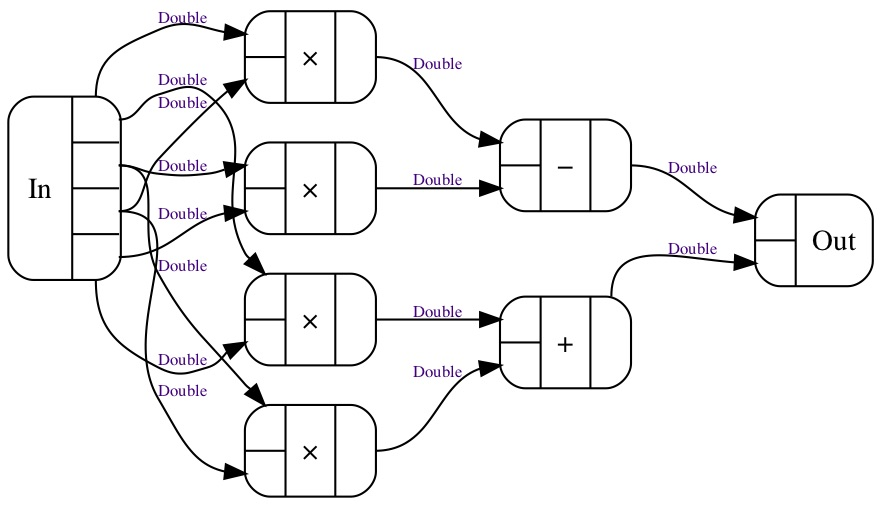
\includegraphics[width=\paperwidth]{graphics/complex-mul.jpg}}
  }

  \begin{frame}
    %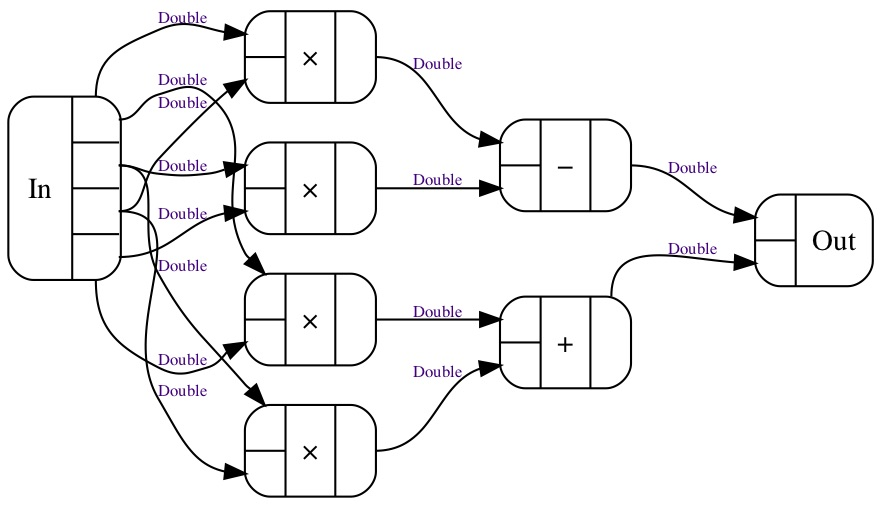
\includegraphics[width=\textwidth]{graphics/complex-mul.jpg}
  \end{frame}

  }

  \begin{frame}
    \begin{center}
      \fontfamily{ugq}
      \Large \color{black}
      How does this work??
    \end{center}
  \end{frame}


  \begin{frame}
    \frametitle{Categorical semantics}
    \begin{center}


      %  \colorbox{green}{
      \begin{minipage}{.9\textwidth}
        The simply-typed lambda calculus is the \textit{internal language} of \textit{Cartesian closed categories}.
      \end{minipage}
      %  }

      \vskip1em

      which means

      \vskip.5em

      %  \colorbox{gray}{
      \begin{minipage}{.9\textwidth}
        We can interpret the lambda calculus in any CCC.
      \end{minipage}
      %  }

    \end{center}
  \end{frame}

  \begin{frame}[fragile]
    \frametitle{Cartesian closed categories}
    A Cartesian closed category is a category with function objects.

    \[
    \mathcal{C}(A \times B, C) \cong \mathcal{C}(A, C^B)
    \]

    In Haskell, this isomorphism is called``curry".

    \begin{code}
      curry :: ((a,b) -> c) -> a -> b -> c
      curry f a b = f (a, b)

      uncurry :: (a -> b -> c) -> (a, b) -> c
      uncurry f (a, b) = f a b
    \end{code}

  \end{frame}


  \section{Categorical semantics}

  \begin{frame}
    \frametitle{Curry-Howard correspondence}
    \begin{figure}
      \begin{minipage}{.5\textwidth}
        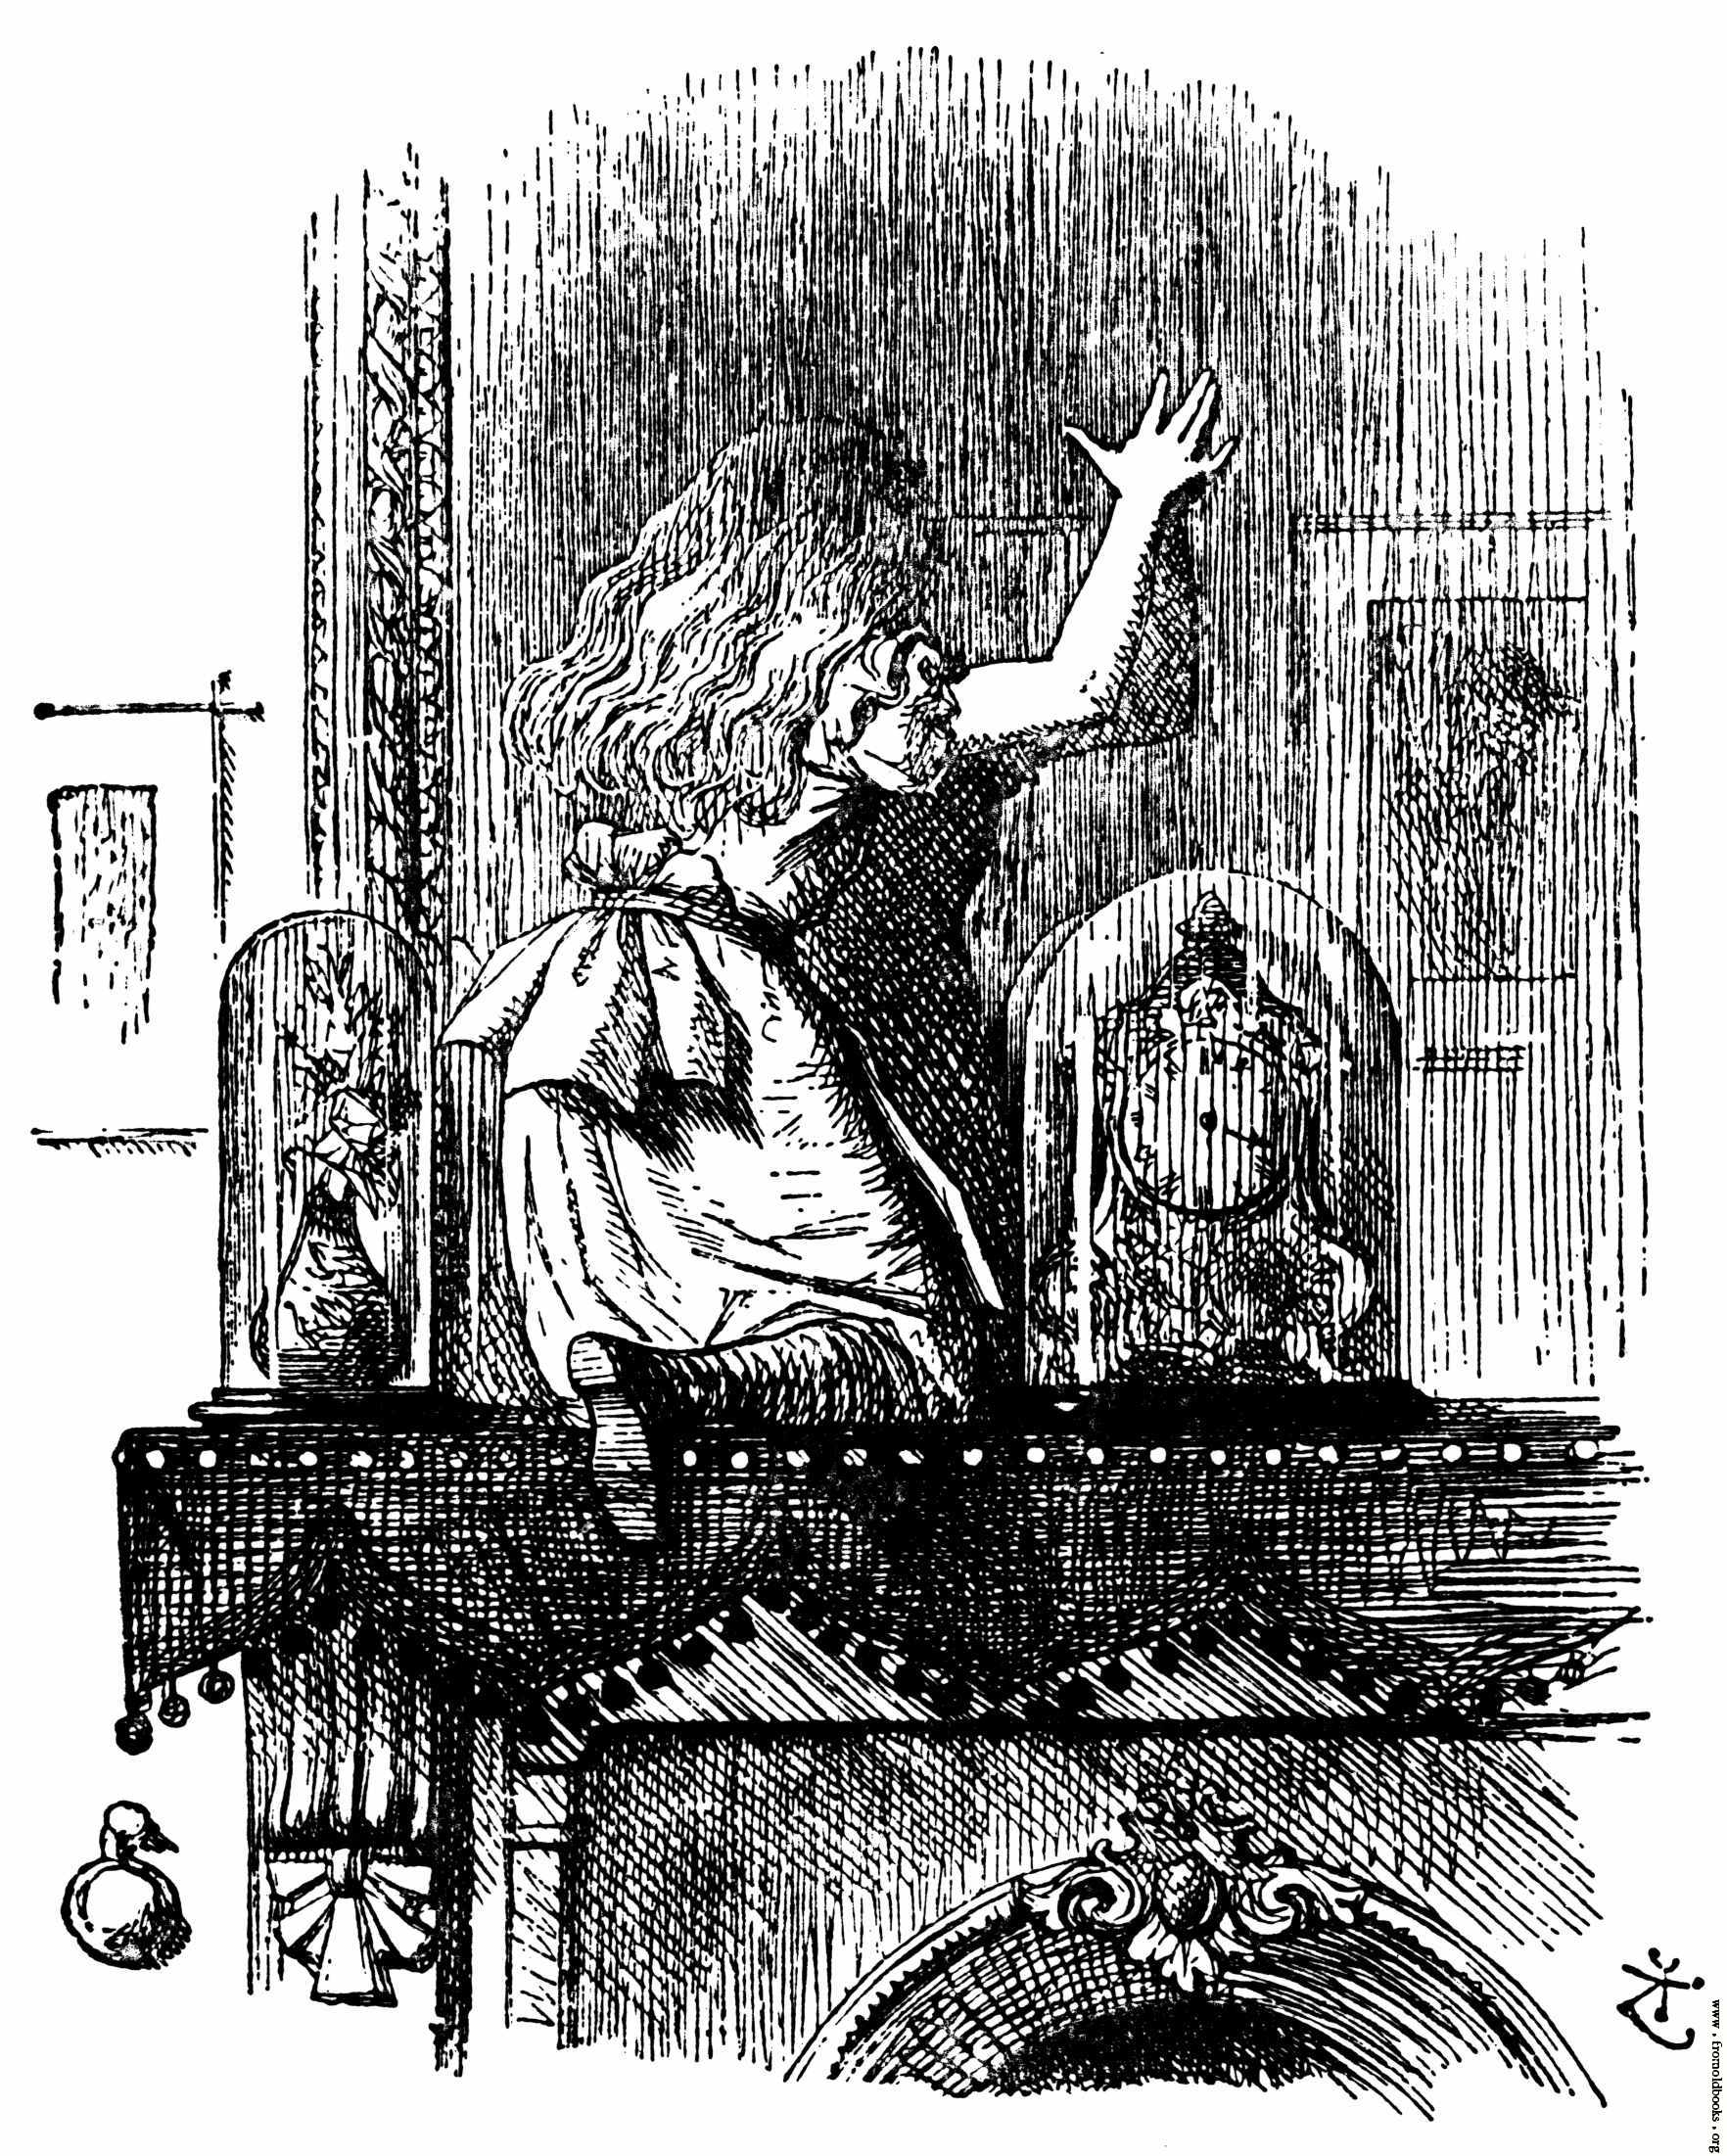
\includegraphics[width=\textwidth]{graphics/011-Into-the-looking-glass-q45-1764x2202.jpg}
        %      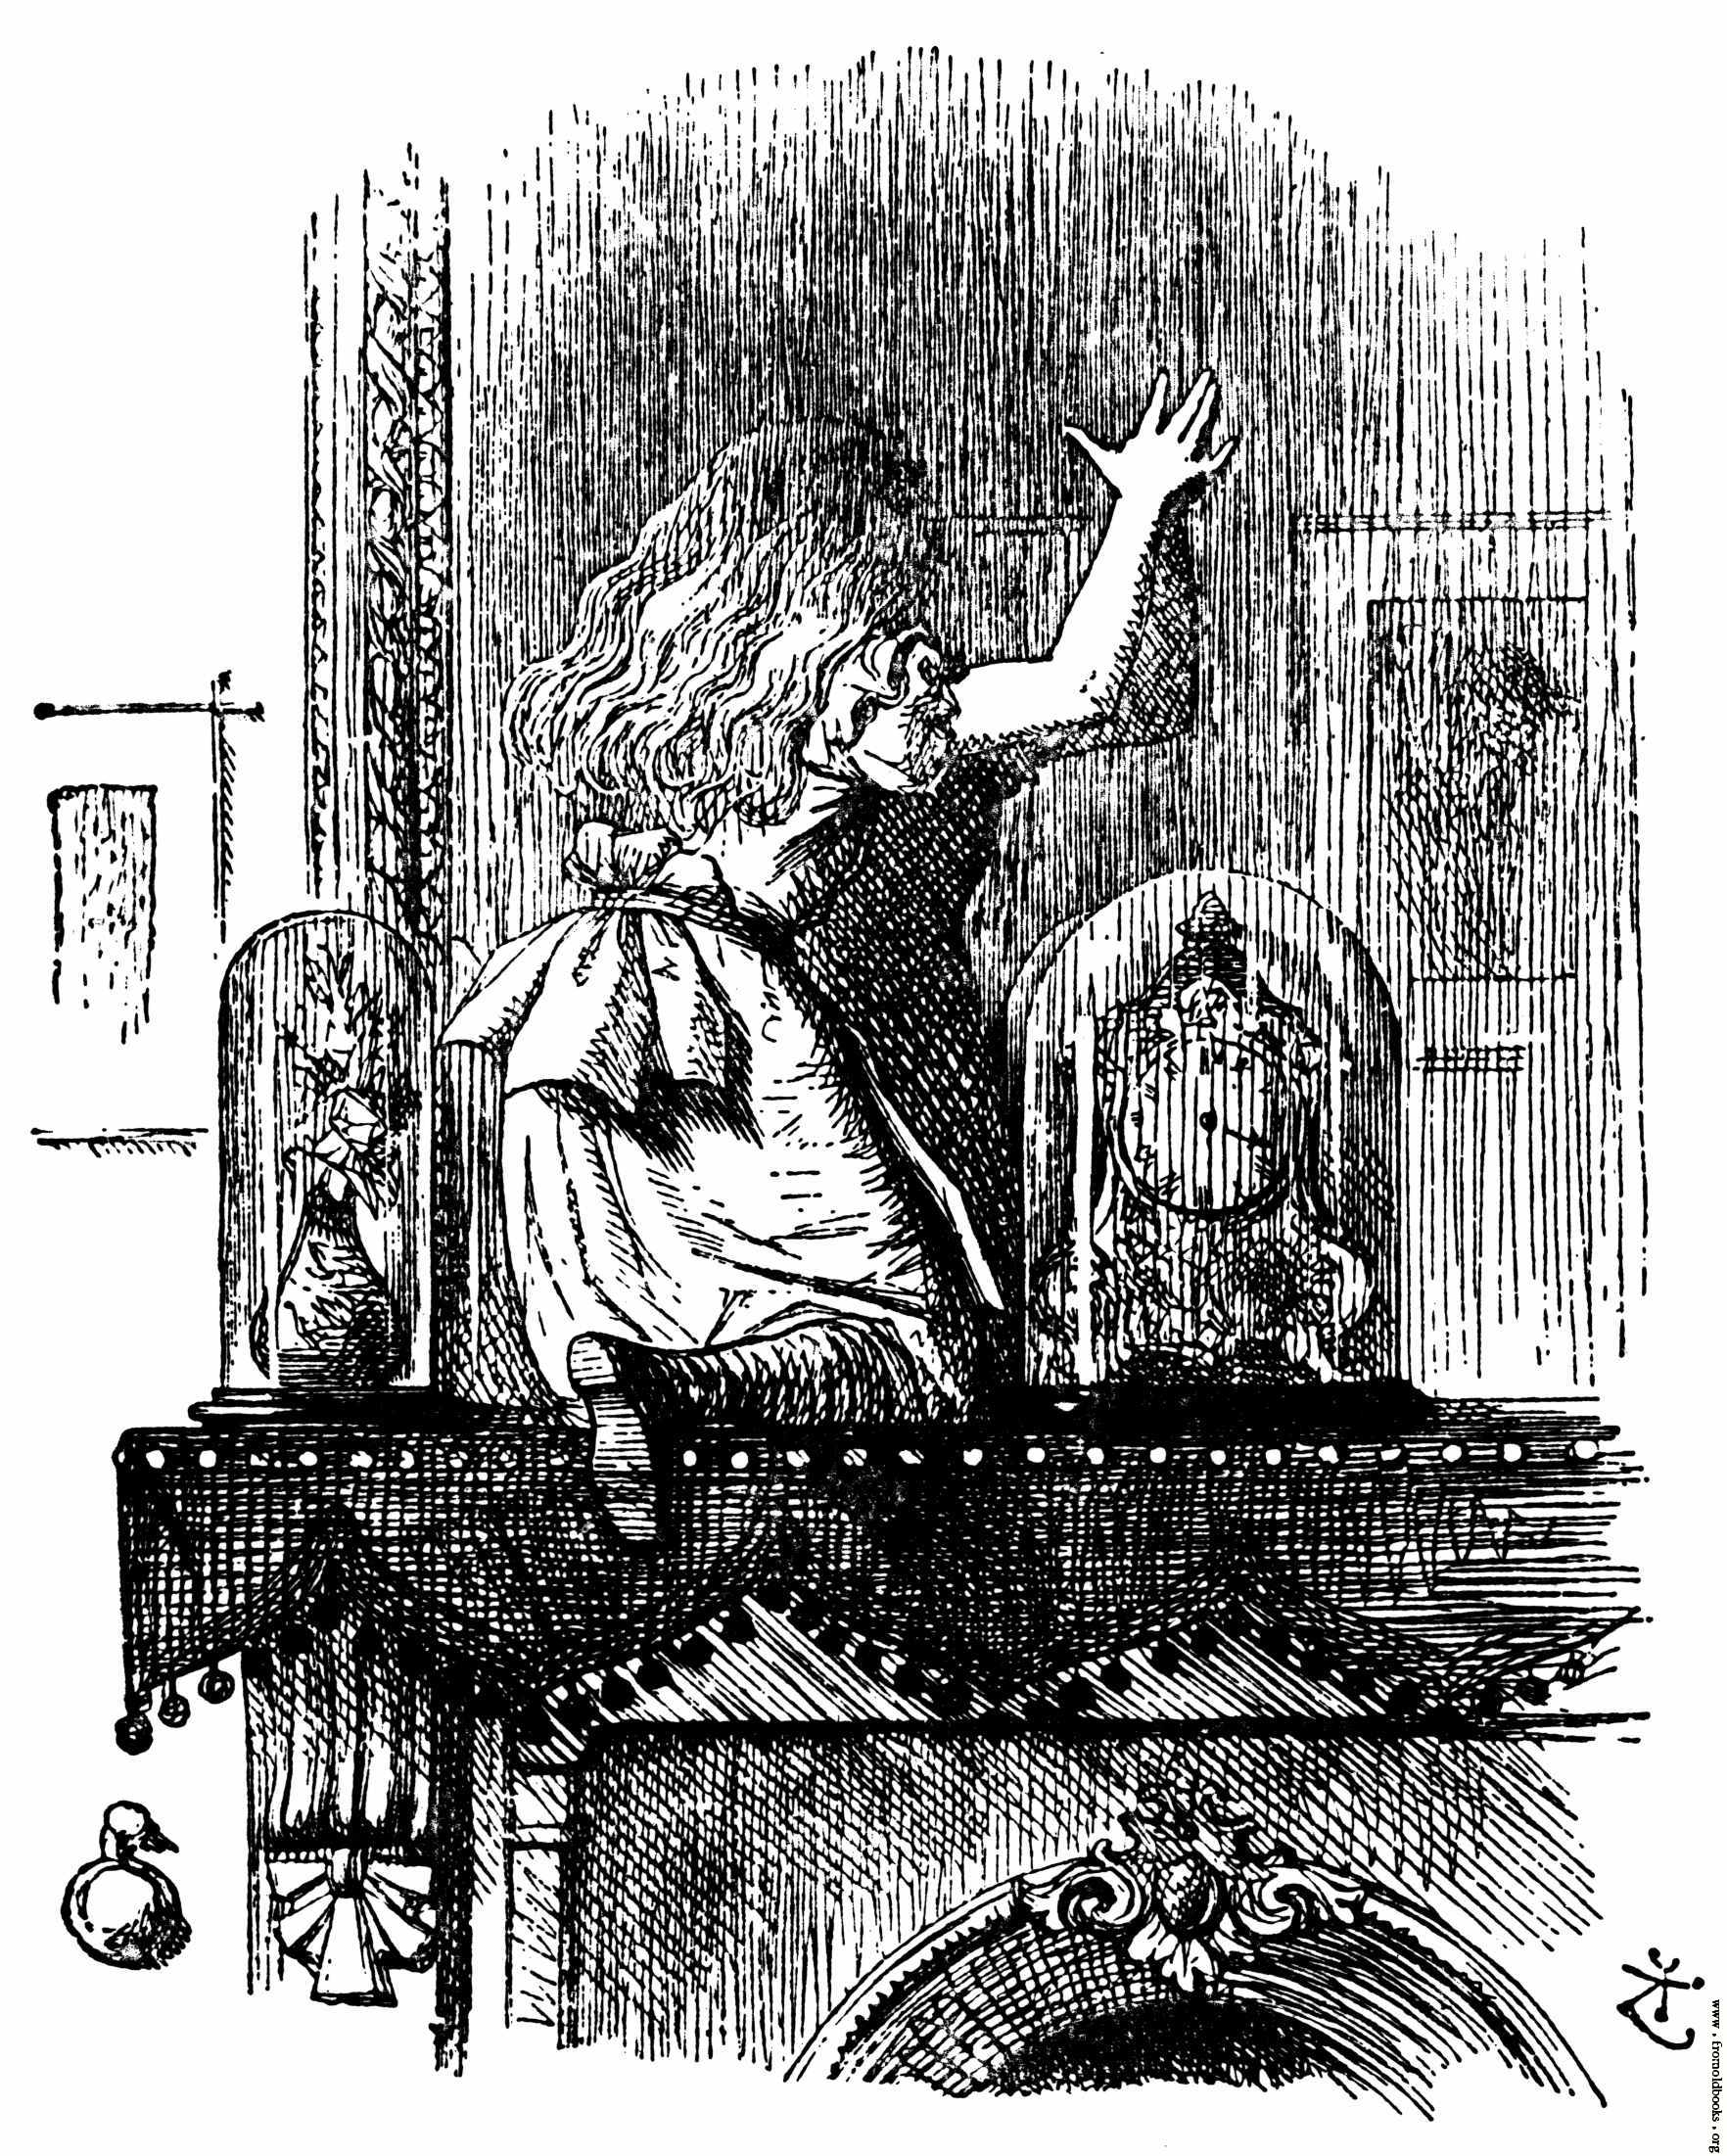
\includegraphics[width=0.5\textwidth]{graphics/011-Into-the-looking-glass-q45-1764x2202.jpg}
      \end{minipage}%
      \begin{minipage}{.5\textwidth}
        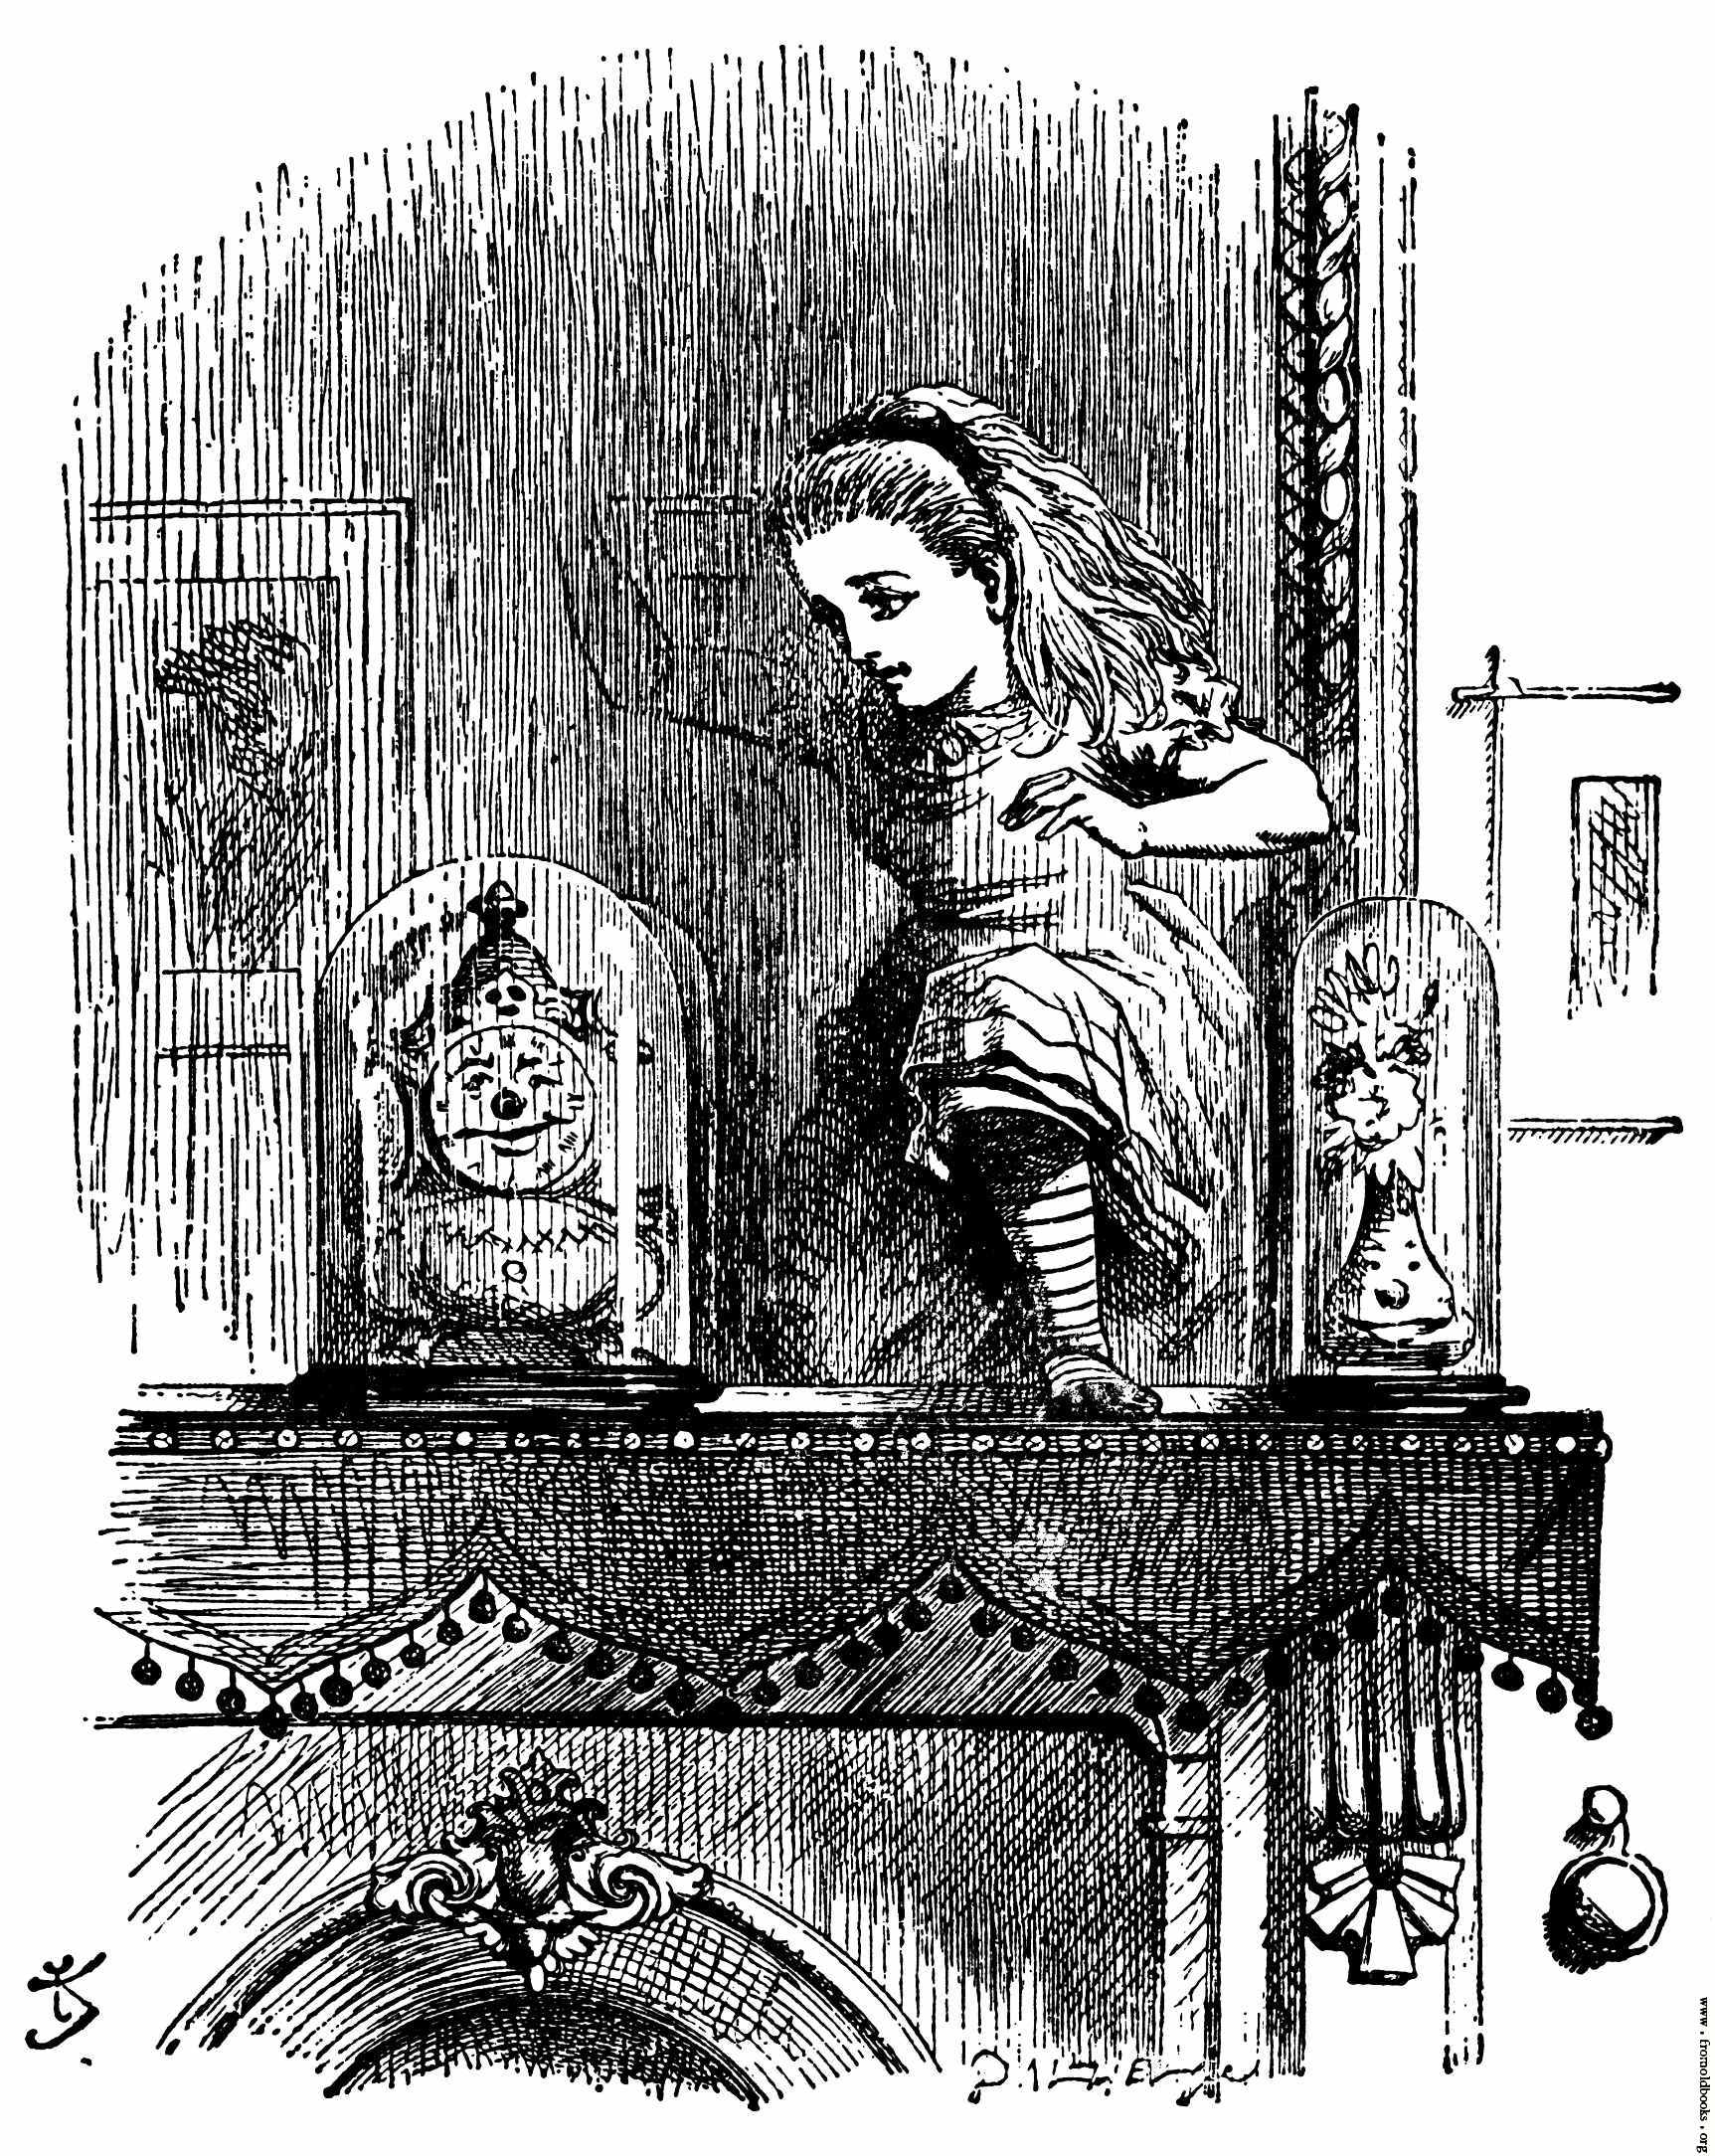
\includegraphics[width=\textwidth]{graphics/013-Alice-emerging-from-the-looking-glass-q42-1725x2168.jpg}
        %      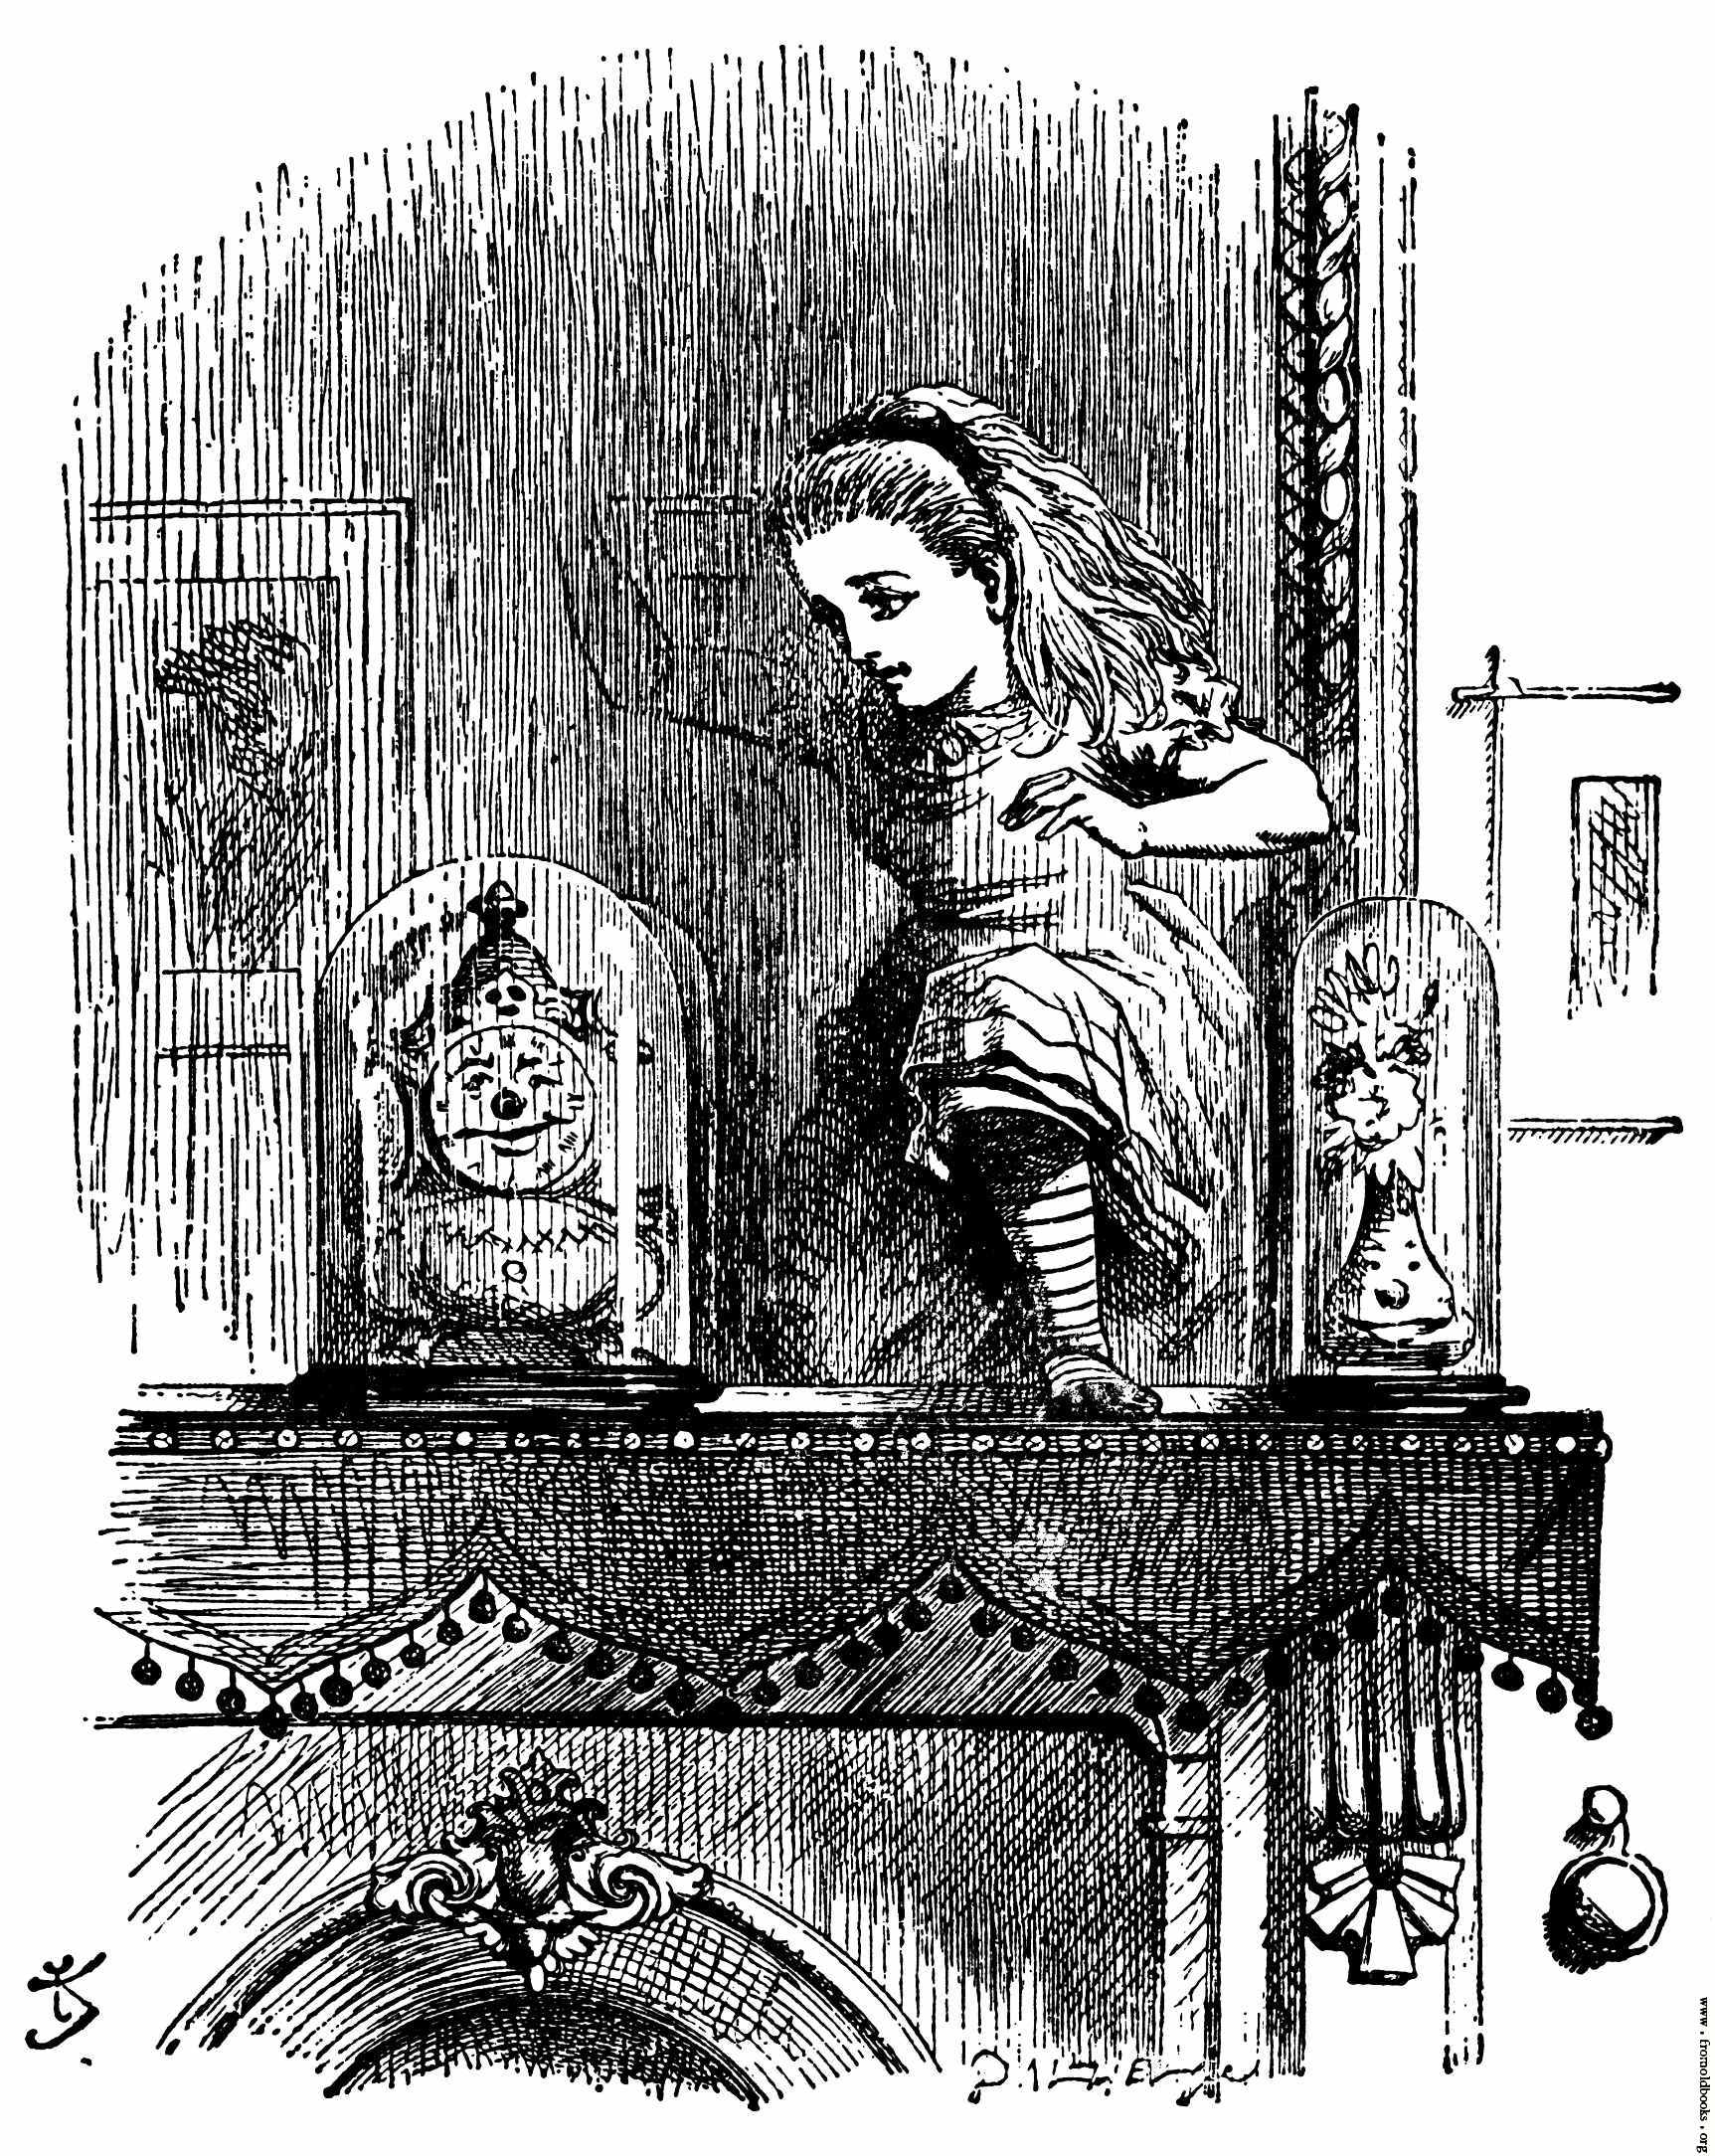
\includegraphics[width=0.5\textwidth]{graphics/013-Alice-emerging-from-the-looking-glass-q42-1725x2168.jpg}
      \end{minipage}

    \end{figure}
  \end{frame}

  \begin{frame}
    \frametitle{Curry-Howard-Lambek correspondence}
    \begin{center}
      % Triangle
      \begin{tikzpicture}[scale=2.7]
        \draw (0,0) -- (90:1);
        \draw (0,0) -- (210:1);
        \draw (0,0) -- (330:1);
        \def\r{4}
        %90 210 330
        %150 270 390=30
        \draw (150:.\r) node {Logic};
        \draw (30:.\r)  node {Types};
        {{\draw (270:.\r) node {Categories};}}
      \end{tikzpicture}
    \end{center}
  \end{frame}

  \begin{frame}[fragile]
    \frametitle{Categorical semantics}

    \begin{center}

      \begin{tikzcd}
        \mathrm{Type~theories}
        \arrow[r, "\mathrm{Syntactic~category}"{name=F}, bend left=25] &
        \mathrm{Categories}
        \arrow[l, "\mathrm{Internal~language}"{name=G}, bend left=25]
        %--- Adjunction Symbol
        \arrow[phantom, from=F, to=G, "\dashv" rotate=-90]
        % \arrow[phantom, from=F, to=G, "\dashv" rotate=-90, no line]
      \end{tikzcd}

    \end{center}

  \end{frame}

  \begin{frame}
    \frametitle{Advantages}

    \begin{itemize}
      \item The internal language is valid in every model
      \item More easily prove properties about a type theory using CT
      \item CT proofs using the internal language can be easier
      \item The CT can illuminate the TT, and vice versa
      \item Can use the internal language to define internal structures
    \end{itemize}
  \end{frame}

  \section{Adjunctions}

  \begin{frame}
    \frametitle{Adjunctions}

    \[
      F \dashv U: \mathcal{C} \rightarrow \mathcal{D}
    \]
    \[
      \begin{tikzcd}
        [ampersand replacement=\&, column sep=large]
        \mathcal{C}
        \arrow[r, "F"{name=F}, bend left=25] \&
        \mathcal{D}
        \arrow[l, "U"{name=G}, bend left=25]
        %--- Adjunction Symbol
        \arrow[phantom, from=F, to=G, "\dashv" rotate=-90]
        % \arrow[phantom, from=F, to=G, "\dashv" rotate=-90, no line]
      \end{tikzcd}
    \]

    \begin{equation*}
      \mathcal{D}(F c, d) \cong \mathcal{C}(c, U d)
    \end{equation*}

    \begin{prooftree}
      \AxiomC{$Fc \rightarrow d$ in $\mathcal{D}$}
      \doubleLine
      \UnaryInfC{$c \rightarrow Ud$ in $\mathcal{C}$}
    \end{prooftree}

  \end{frame}

  \begin{frame}
    \frametitle{Example: free monoid}

    The free monoid on an alphabet $\Lambda$ is the set $\Lambda^\ast$ of words in $\Lambda$.

    \begin{prooftree}
      \AxiomC{$\Lambda^\ast \rightarrow m$ in $\cat{Mon}$}
      \doubleLine
      \UnaryInfC{$\Lambda \rightarrow m$ in $\cat{Set}$}
    \end{prooftree}

    Why?

    A monoid homomorphism has to respect multiplication, so

    \[
      f(abcd\cdots) = f(a) f(b) f(c) \cdots
    \]

  \end{frame}

  % \begin{frame}
  %   \frametitle{Example: vector space}

  % Given a set $S$, we can make a vector space with that set as basis.
  % \begin{prooftree}
  % \AxiomC{$\mathbb{R}S \rightarrow V$ in $\cat{Vect}$}
  % \doubleLine
  % \UnaryInfC{$S \rightarrow V$ in $\cat{Set}$}
  % \end{prooftree}

  % A linear map is determined by its action on a basis.

  % \end{frame}

  \begin{frame}[fragile]
    \frametitle{Example: currying}

    The functor $- \times b$ is left adjoint to $(-)^b$.

    \begin{prooftree}
      \AxiomC{$a \times b \rightarrow c$ in $\cat{Type}$}
      \doubleLine
      \UnaryInfC{$a \rightarrow c^b$ in $\cat{Type}$}
    \end{prooftree}

    \vskip1em

    \begin{code}
      curry :: ((a,b) -> c) -> a -> b -> c
      curry f a b = f (a, b)

      uncurry :: (a -> b -> c) -> (a, b) -> c
      uncurry f (a, b) = f a b
    \end{code}

  \end{frame}

  \begin{frame}
    \frametitle{Example: quantifiers $\exists_y \dashv w_y \dashv \forall_y$ }
    \begin{align*}
      w_y : \Formulae(\bar x) &\to \Formulae(\bar x, y) \\
      \phi(\bar x) &\mapsto \phi(\bar x)
    \end{align*}

    \begin{prooftree}
      \AxiomC{$\bar x, y \vdash w_y\phi(\bar x) \Rightarrow \psi(\bar x, y)$}
      \doubleLine
      \UnaryInfC{$\bar x\vdash \phi(\bar x) \Rightarrow \forall_y\psi(\bar x, y)$}
    \end{prooftree}

    \begin{prooftree}
      \AxiomC{$\bar x \vdash \exists_y\psi(\bar x, y) \Rightarrow \phi(\bar x) $}
      \doubleLine
      \UnaryInfC{$\bar x, y \vdash \psi(\bar x, y) \Rightarrow w_y\phi(\bar x) $}
    \end{prooftree}

  \end{frame}

  \begin{frame}
    \frametitle{Compiling to CCCs}
    \begin{itemize}
      \item Categorical semantics for STLC in CCCs
      \item Lots of CCCs
      \item GHC Core's System FC can (mostly) be converted to STLC
      \item GHC plugin, rewrite rules
      \item Convert Haskell src to VHDL, diagrams, etc
    \end{itemize}
  \end{frame}

  \begin{frame}{}
    \begin{center}
      % \fontfamily{ugq}
      \Large \color{black} There's more to type theory than STLC!
    \end{center}
  \end{frame}

  \begin{frame}
    \frametitle{}
    \begin{itemize}
      \item polymorphic types
      \item existential types
      \item universal types
      \item type classes
      \item union and intersection types
      \item quotient types
      \item dependent types
      \item refinement types
      \item homotopy type theory
      \item \ldots
    \end{itemize}
  \end{frame}

  \section{Dependent types}

  \begin{frame}
    \frametitle{Dependent types}
    A dependent type is one that contains free variables.

    \[
      \tau : \mathrm{Type} \;\;\; x: \tau \vdash P(x) : \mathrm{Type}
    \]

    It \textit{depends on} terms.

  \end{frame}

  \begin{frame}[fragile]
    \frametitle{Dependent types}

    \begin{align*}
      n: \mathrm{Nat} & \;\vdash\; \mathrm{IsEven}\,n : \mathrm{Type}
    \end{align*}

    \vskip2em

    \begin{code}
      data IsEven (n : Nat) : Type where
        ZEven : IsEven 0
        SSEven : IsEven n -> IsEven (n + 2)
    \end{code}

  \end{frame}


  \begin{frame}[fragile]
    \frametitle{Dependent types}

    \begin{align*}
      n: \mathrm{Nat}, a : \mathrm{Type} & \;\vdash\; \mathrm{Vect}_n(a) : \mathrm{Type}
    \end{align*}

    \vskip2em

    \begin{code}
      data Vect (n : Nat) (a : Type) : Type where
        Nil : Vect 0 a
        (::) : a -> Vect n a -> Vect (n + 1) a
    \end{code}

  \end{frame}

  \begin{frame}[fragile]
    \frametitle{Dependent product type}

    \begin{center}

    \begin{code}
          replicate : (n : Nat) -> a -> Vect n a
    \end{code}

    \begin{align*}
      \operatorname{replicate} &: \prod_{a : \Type} \prod_{n : \mathbb{N}} \prod_{x : a} \Vect_n(a) \\
      &=  \prod_{a : \Type} \prod_{n : \mathbb{N}} a \to \Vect_n(a)
    \end{align*}

      \[
        a \to b :\equiv \prod_{\_\, : a} b
      \]

    \end{center}
  \end{frame}

  \begin{frame}[fragile]
    \frametitle{Dependent sum type}

    \begin{center}

    \begin{code}
evenLenLists = (l : List Int ** m : Nat ** length l = 2 * m)
    \end{code}

      \begin{align*}
        \operatorname{evenLenLists} = \sum_{l : \List(\Int)} \sum_{m:\N} \operatorname{length}(l) = 2m
      \end{align*}

      \[
        (a, b) :\equiv \sum_{\_ \,: a} b
      \]

    \end{center}
  \end{frame}

  \begin{frame}
    Dependent types are the internal language of \textit{locally Cartesian closed categories}.
  \end{frame}

  \section{Semantics}

  \begin{frame}
    \frametitle{Semantics}
    Objects: closed types

    Arrows: terms in context

    also arrows: functions
    \begin{align*}
      f &: a \to b \\
      [\![f]\!]  &: [\![a]\!] \to [\![b]\!]
    \end{align*}
  \end{frame}

  \begin{frame}
    \frametitle{Semantics for dependent types}
    \begin{align*}
      \IsEven&: \N \to \Set  \\
      \IsEven &\, 0 = \{ \textrm{zeroEven} \} \\
      \IsEven &\, 1 = \{ \textrm{} \} \\
      \IsEven &\, 2 = \{ \textrm{twoEven} \} \\
      \IsEven &\, 3 = \{ \textrm{} \} \\
      \IsEven &\, 4 = \{ \textrm{fourEven} \} \\
      &\vdots
    \end{align*}
  \end{frame}

  \begin{frame}
    \frametitle{Semantics for dependent types}
    \begin{align*}
      \CustomerOf&: \Bank \to \Set  \\
      \CustomerOf& \ANZ = \{ \textrm{Alice, Albert, Anne-Marie} \} \\
      \CustomerOf& \CBA = \{ \textrm{Calvin, Colin} \} \\
      \CustomerOf& \NAB = \{ \textrm{Nathan} \} \\
      \CustomerOf& \Westpac = \{ \textrm{Wendy, Will} \} \\
    \end{align*}

  \end{frame}

  \begin{frame}
    \frametitle{Thinking backwards}
    \begin{minipage}{.5\textwidth}
      \begin{align*}
        p : \IsEven \_  &\to \N\\
        p \, zeroEven &= 0 \\
        p \, twoEven &= 2 \\
        p \, fourEven &= 4 \\
        &\vdots
      \end{align*}

    \end{minipage}% This must go next to `\end{minipage}`
    \begin{minipage}{.5\textwidth}
      \begin{align*}
        p : \CustomerOf \_       &\to \Bank\\
        p \, \textrm{Alice}      &= \ANZ \\
        p \, \textrm{Albert}     &= \ANZ \\
        p \, \textrm{Anne-Marie} &= \ANZ \\
        p \, \textrm{Calvin}     &= \CBA \\
        p \, \textrm{Colin}      &= \CBA \\
        p \, \textrm{Nathan}     &= \NAB \\
        p \, \textrm{Wendy}      &= \Westpac \\
        p \, \textrm{Will}       &= \Westpac \\
      \end{align*}
    \end{minipage}
  \end{frame}



  \begin{frame}
    \frametitle{Semantics for dependent types}

    \begin{center}

      \begin{tikzpicture}[scale=.5]
        \begin{scope}
          \def\x{2}
          \begin{scope}[yshift=7.5cm]
            \node at (\x, 1) {\vdots};
          \end{scope}
          \begin{scope}[yshift=6cm]
            \draw [fill=yellow] (0,0.5) rectangle (4, 1.5);
            \node[right] at (\x+2, 1) {4};
            \node at (\x, 1) {fourEven};
          \end{scope}
          \begin{scope}[yshift=4.5cm]
            \draw [fill=yellow] (0,0.5) rectangle (4, 1.5);
            \node[right] at (\x+2, 1) {3};
          \end{scope}
          \begin{scope}[yshift=3cm]
            \draw [fill=yellow] (0,0.5) rectangle (4, 1.5);
            \node[right] at (\x+2, 1) {2};
            \node at (\x, 1) {twoEven};
          \end{scope}
          \begin{scope}[yshift=1.5cm]
            \draw [fill=yellow] (0,0.5) rectangle (4, 1.5);
            \node[right] at (\x+2, 1) {1};
          \end{scope}
          \begin{scope}[yshift=0]
            \draw [fill=yellow] (0,0.5) rectangle (4, 1.5);
            \node[right] at (\x+2, 1) {0};
            \node at (\x, 1) {zeroEven};
          \end{scope}

          \node at (\x,-1) {$\Set\!/\N$};
        \end{scope}
        \begin{scope}[xshift=10cm]
          \def\x{2}
          \begin{scope}[yshift=6.5cm]
            \draw [fill=yellow] (0,0.5) rectangle (4, 3.5);
            \node[right] at (\x+2, 3) {ANZ};
            \node at (\x, 3) {Alice};
            \node at (\x, 2) {Albert};
            \node at (\x, 1) {Anne-Marie};
          \end{scope}
          \begin{scope}[yshift=4cm]
            \draw [fill=yellow] (0,0.5) rectangle (4, 2.5);
            \node[right] at (\x+2, 2) {CBA};
            \node at (\x, 2) {Calvin};
            \node at (\x, 1) {Colin};
          \end{scope}
          \begin{scope}[yshift=2.5cm]
            \draw [fill=yellow] (0,0.5) rectangle (4, 1.5);
            \node[right] at (\x+2, 1) {NAB};
            \node at (\x, 1) {Nathan};
          \end{scope}
          \begin{scope}[yshift=0cm]
            \draw [fill=yellow] (0,0.5) rectangle (4, 2.5);
            \node[right] at (\x+2, 2) {Westpac};
            \node at (\x, 2) {Wendy};
            \node at (\x, 1) {Will};
          \end{scope}

          \node at (\x,-1) {$\Set\!/\Bank$};
        \end{scope}
      \end{tikzpicture}

    \end{center}
  \end{frame}

  \begin{frame}[fragile]
    \frametitle{Over-categories}

    \[
      X \in \mathcal{C}, \mathcal{C}/X
    \]

    \begin{minipage}{\textwidth}
      \begin{minipage}{.5\textwidth}
        Objects:
        \begin{tikzcd}[ampersand replacement=\&]
          A \arrow{d}{p} \\
          X
        \end{tikzcd}

        Arrows:
        \begin{tikzcd}[ampersand replacement=\&]
          A \arrow{rr}{f} \arrow{dr}{p} \&\& \arrow{dl}{q} B \\
          \& X
        \end{tikzcd}
      \end{minipage}%
      \begin{minipage}{.5\textwidth}
        fibre $(A)_x = p^{-1} x$ in $\Set$

        \vskip1em
        section $s: X \to A$
        \\
        such that $p \circ s = \operatorname{id}$
      \end{minipage}
    \end{minipage}


  \end{frame}

  \begin{frame}
    \frametitle{Over-categories}
    \begin{minipage}{\textwidth}
      \begin{minipage}{.5\textwidth}
        \begin{tikzpicture}[scale=.5]
          \def\x{2}
          \begin{scope}[yshift=6.5cm]
            \draw [fill=yellow] (0,0.5) rectangle (4, 3.5);
            \node[right] at (\x+2, 3) {ANZ};
            \node at (\x, 3) {Alice};
            \node at (\x, 2) {Albert};
            \node at (\x, 1) {Anne-Marie};
          \end{scope}
          \begin{scope}[yshift=4cm]
            \draw [fill=yellow] (0,0.5) rectangle (4, 2.5);
            \node[right] at (\x+2, 2) {CBA};
            \node at (\x, 2) {Calvin};
            \node at (\x, 1) {Colin};
          \end{scope}
          \begin{scope}[yshift=2.5cm]
            \draw [fill=yellow] (0,0.5) rectangle (4, 1.5);
            \node[right] at (\x+2, 1) {NAB};
            \node at (\x, 1) {Nathan};
          \end{scope}
          \begin{scope}[yshift=0cm]
            \draw [fill=yellow] (0,0.5) rectangle (4, 2.5);
            \node[right] at (\x+2, 2) {Westpac};
            \node at (\x, 2) {Wendy};
            \node at (\x, 1) {Will};
          \end{scope}
        \end{tikzpicture}
      \end{minipage}%
      \begin{minipage}{.5\textwidth}
        \begin{tikzpicture}[scale=.5]
          \def\x{2}
          \begin{scope}[yshift=7.5cm]
            \draw [fill=yellow] (0,0.5) rectangle (4, 3.5);
            \node[right] at (\x+2, 3) {ANZ};
            \node at (\x, 3) {Artarmon};
            \node at (\x, 2) {Annandale};
            \node at (\x, 1) {Auburn};
          \end{scope}
          \begin{scope}[yshift=5cm]
            \draw [fill=yellow] (0,0.5) rectangle (4, 2.5);
            \node[right] at (\x+2, 2) {CBA};
            \node at (\x, 2) {Clovelly};
            \node at (\x, 1) {Curl Curl};
          \end{scope}
          \begin{scope}[yshift=2.5cm]
            \draw [fill=yellow] (0,0.5) rectangle (4, 2.5);
            \node[right] at (\x+2, 2) {NAB};
            \node at (\x, 2) {Naremburn};
            \node at (\x, 1) {Nth Bondi};
          \end{scope}
          \begin{scope}[yshift=0cm]
            \draw [fill=yellow] (0,0.5) rectangle (4, 2.5);
            \node[right] at (\x+2, 2) {Westpac};
            \node at (\x, 2) {Wahroonga};
            \node at (\x, 1) {Woollahra};
          \end{scope}
        \end{tikzpicture}
      \end{minipage}
    \end{minipage}

    fibre $(A)_x = p^{-1} x$

    section $s: X \to A$ such that $p \circ s = \operatorname{id}$
  \end{frame}

  \begin{frame}
    \frametitle{Substitution}
    \[ \bankOf: \Branch \to \Bank \]

    \[ b : \Bank \vdash \CustomerOf b : \Type \]
    \[ br : \Branch \vdash \CustomerOf (\bankOf br) : \Type \]
  \end{frame}


  \begin{frame}
    \begin{center}
      \begin{tikzpicture}[scale=.5]
        \def\x{2}
        \begin{scope}[yshift=13cm]
          \draw [fill=yellow] (0,0.5) rectangle (4, 2.5);
          \node[right] at (\x+2, 2) {Artarmon};
          \node at (\x, 2) {Alice};
          \node at (\x, 1) {Albert};
        \end{scope}
        \begin{scope}[yshift=11.5cm]
          \draw [fill=yellow] (0,0.5) rectangle (4, 1.5);
          \node[right] at (\x+2, 1) {Annandale};
        \end{scope}
        \begin{scope}[yshift=10cm]
          \draw [fill=yellow] (0,0.5) rectangle (4, 1.5);
          \node[right] at (\x+2, 1) {Auburn};
          \node at (\x, 1) {Anne-Marie};
        \end{scope}
        \begin{scope}[yshift=7.5cm]
          \draw [fill=yellow] (0,0.5) rectangle (4, 2.5);
          \node[right] at (\x+2, 2) {Clovelly};
          \node at (\x, 2) {Calvin};
          \node at (\x, 1) {Colin};
        \end{scope}
        \begin{scope}[yshift=6cm]
          \draw [fill=yellow] (0,0.5) rectangle (4, 1.5);
          \node[right] at (\x+2, 1) {Curl Curl};
        \end{scope}
        \begin{scope}[yshift=4.5cm]
          \draw [fill=yellow] (0,0.5) rectangle (4, 1.5);
          \node[right] at (\x+2, 1) {Naremburn};
        \end{scope}
        \begin{scope}[yshift=3cm]
          \draw [fill=yellow] (0,0.5) rectangle (4, 1.5);
          \node[right] at (\x+2, 1) {Nth Bondi};
          \node at (\x, 1) {Nathan};
        \end{scope}
        \begin{scope}[yshift=1.5cm]
          \draw [fill=yellow] (0,0.5) rectangle (4, 1.5);
          \node[right] at (\x+2, 1) {Wahroonga};
          \node at (\x, 1) {Will};
        \end{scope}
        \begin{scope}[yshift=0cm]
          \draw [fill=yellow] (0,0.5) rectangle (4, 1.5);
          \node[right] at (\x+2, 1) {Woollahra};
          \node at (\x, 1) {Wendy};
        \end{scope}
      \end{tikzpicture}\frametitle{}
    \end{center}
  \end{frame}

  \begin{frame}
    \begin{center}
      \begin{tikzpicture}[scale=.5]
        \def\x{2}
        \begin{scope}[yshift=6cm]
          \node at (\x, 1) {\vdots};
        \end{scope}
        \begin{scope}[yshift=4.5cm]
          \draw [fill=yellow] (0,0.5) rectangle (4, 1.5);
          \node[right] at (\x+2, 1) {``hello"};
          %        \node at (\x, 1) {};
        \end{scope}
        \begin{scope}[yshift=3cm]
          \draw [fill=yellow] (0,0.5) rectangle (4, 1.5);
          \node[right] at (\x+2, 1) {``no"};
          \node at (\x, 1) {twoEven};
        \end{scope}
        \begin{scope}[yshift=1.5cm]
          \draw [fill=yellow] (0,0.5) rectangle (4, 1.5);
          \node[right] at (\x+2, 1) {``icecream"};
          \node at (\x, 1) {eightEven};
        \end{scope}
        \begin{scope}[yshift=0cm]
          \draw [fill=yellow] (0,0.5) rectangle (4, 1.5);
          \node[right] at (\x+2, 1) {``submarine"};
        \end{scope}
        \begin{scope}[yshift=-1cm]
          \node at (\x, 1) {\vdots};
        \end{scope}
      \end{tikzpicture}\frametitle{}

      \[
        s : \String \vdash \IsEven (\length s) : \Type
      \]
    \end{center}
  \end{frame}

  \begin{frame}[fragile]
    \frametitle{Substitution = pullback aka change of base}

    \begin{align*}
      \bankOf &: \Branch \to \Bank \\
      \bankOf^\ast &: \Set/\Bank \to \Set/\Branch
    \end{align*}


  \end{frame}

  \begin{frame}[fragile]
    \frametitle{Substitution = pullback aka change of base}

    \[
      \begin{tikzcd}
        [ampersand replacement=\&]
        T \arrow[bend left]{drr}{f}
        \arrow[bend right,swap]{ddr}{g}
        \arrow[dashed]{dr}[description]{\exists !} \& \& \\
        \& \Branch\times_{\Bank} \Customer \arrow{r} \arrow{d}{p^\ast} \& \Customer \arrow{d}{p} \\
        \& \Branch \arrow{r}{\bankOf} \& \Bank
      \end{tikzcd}
    \]

    \begin{align*}
      \Branch\times_{\Bank} \Customer
      &=
      \bankOf^\ast \Customer
      \\
      &= \left\{ (br, c) \middle| \bankOf(br) = p(c)\right\}
    \end{align*}

  \end{frame}

  \begin{frame}
    \frametitle{Dependent sum}
    \begin{center}

      \[
        f : X \to Y
      \]
      \[
        \sum_f: \Set/X \to \Set/Y
      \]

      \begin{tikzcd}[ampersand replacement=\&]
        A \arrow{d}{p} \\
        X \arrow{d}{f} \\
        Y
      \end{tikzcd}

      \[
        \sum_f \dashv f^\ast
      \]

    \end{center}
  \end{frame}

  \begin{frame}
    \frametitle{$\sum_{x:X} := \sum_{!_X} \quad !_X: X \to \ast$}

    \begin{center}
      \[
        \Set/\!\ast(\sum_f p, q) \cong \Set/X(p, f^\ast q)
      \]

      \begin{minipage}{.5\textwidth}
        \begin{tikzpicture}[scale=.5]
          \def\x{2}
          \begin{scope}
            \begin{scope}[yshift=0]
              \draw [fill=yellow] (0,0.5) rectangle (4, 6.5);
              \node[right] at (\x+2, 6) {$\ast$};
              \node at (\x, 6) {\vdots};
              \node at (\x, 5) {eightEven};
              \node at (\x, 4) {sixEven};
              \node at (\x, 3) {fourEven};
              \node at (\x, 2) {twoEven};
              \node at (\x, 1) {zeroEven};
            \end{scope}
          \end{scope}
          \begin{scope}[xshift=5cm]
            \begin{scope}[yshift=0]
              \draw [fill=yellow] (0,0.5) rectangle (4, 3.5);
              \node[right] at (\x+2, 3) {$\ast$};
              \node at (\x, 3) {apple};
              \node at (\x, 2) {banana};
              \node at (\x, 1) {cherry};
            \end{scope}
          \end{scope}
        \end{tikzpicture}

      \end{minipage}% This must go next to `\end{minipage}`
      \begin{minipage}{.5\textwidth}
        \begin{tikzpicture}[scale=.5]
          \def\x{2}
          \begin{scope}
            \begin{scope}[yshift=7.5cm]
              \node at (\x, 1) {\vdots};
            \end{scope}
            \begin{scope}[yshift=6cm]
              \draw [fill=yellow] (0,0.5) rectangle (4, 1.5);
              \node[right] at (\x+2, 1) {4};
              \node at (\x, 1) {fourEven};
            \end{scope}
            \begin{scope}[yshift=4.5cm]
              \draw [fill=yellow] (0,0.5) rectangle (4, 1.5);
              \node[right] at (\x+2, 1) {3};
            \end{scope}
            \begin{scope}[yshift=3cm]
              \draw [fill=yellow] (0,0.5) rectangle (4, 1.5);
              \node[right] at (\x+2, 1) {2};
              \node at (\x, 1) {twoEven};
            \end{scope}
            \begin{scope}[yshift=1.5cm]
              \draw [fill=yellow] (0,0.5) rectangle (4, 1.5);
              \node[right] at (\x+2, 1) {1};
            \end{scope}
            \begin{scope}[yshift=0]
              \draw [fill=yellow] (0,0.5) rectangle (4, 1.5);
              \node[right] at (\x+2, 1) {0};
              \node at (\x, 1) {zeroEven};
            \end{scope}
          \end{scope}
          \begin{scope}[xshift=5cm]
            \begin{scope}[yshift=7.5cm]
              \node at (\x, 1) {\vdots};
            \end{scope}
            \begin{scope}[yshift=6cm]
              \draw [fill=yellow] (0,0.5) rectangle (4, 1.5);
              \node[right] at (\x+2, 1) {4};
              \node at (\x, 1) {a b c};
            \end{scope}
            \begin{scope}[yshift=4.5cm]
              \draw [fill=yellow] (0,0.5) rectangle (4, 1.5);
              \node[right] at (\x+2, 1) {3};
              \node at (\x, 1) {a b c};
            \end{scope}
            \begin{scope}[yshift=3cm]
              \draw [fill=yellow] (0,0.5) rectangle (4, 1.5);
              \node[right] at (\x+2, 1) {2};
              \node at (\x, 1) {a b c};
            \end{scope}
            \begin{scope}[yshift=1.5cm]
              \draw [fill=yellow] (0,0.5) rectangle (4, 1.5);
              \node[right] at (\x+2, 1) {1};
              \node at (\x, 1) {a b c};
            \end{scope}
            \begin{scope}[yshift=0]
              \draw [fill=yellow] (0,0.5) rectangle (4, 1.5);
              \node[right] at (\x+2, 1) {0};
              \node at (\x, 1) {a b c};
            \end{scope}
          \end{scope}
        \end{tikzpicture}
      \end{minipage}

    \end{center}
  \end{frame}


  \begin{frame}
    \frametitle{$\sum_{\bankOf}: \Set/\Branch \to \Set/\Bank$}
    \begin{center}

      \begin{tikzpicture}[scale=.4]
        %    \begin{tikzpicture}[xscale=.25,yscale=.5]
        \def\x{2}
        \begin{scope}[xshift=0]
          \begin{scope}[xshift=0]%staff
            \begin{scope}[yshift=10cm]
              \draw [fill=yellow] (0,0.5) rectangle (4, 5.5);
              %            \node[right] at (\x+2, 2) {Artarmon};
              \node at (\x-.5, 5) {\smiley};
              \node at (\x+.5, 5) {\smiley};
              \node at (\x, 4.5) {\smiley};
              \node at (\x-.5, 4) {\smiley};
              \node at (\x+.5, 4) {\smiley};
              %            \node[right] at (\x+2, 1) {Annandale};
              \node at (\x-.5, 2.5) {\smiley};
              \node at (\x+.5, 2.5) {\smiley};
              %            \node[right] at (\x+2, 1) {Auburn};
              \node at (\x-.5, 1) {\smiley};
              \node at (\x+.5, 1) {\smiley};
            \end{scope}
            \begin{scope}[yshift=6cm]
              \draw [fill=yellow] (0,0.5) rectangle (4, 4);
              %            \node[right] at (\x+2, 2) {CBA};
              %            \node[right] at (\x+2, 2) {Clovelly};
              \node at (\x, 3.5) {\smiley};
              \node at (\x, 2.5) {\smiley};
              %            \node[right] at (\x+2, 1) {Curl Curl};
              \node at (\x-.5, 1) {\smiley};
              \node at (\x+.5, 1) {\smiley};
            \end{scope}
            \begin{scope}[yshift=3cm]
              \draw [fill=yellow] (0,0.5) rectangle (4, 3);
              %            \node[right] at (\x+2, 1) {Naremburn};
              \node at (\x, 2.5) {\smiley};
              %            \node[right] at (\x+2, 1) {Nth Bondi};
              \node at (\x-.5, 1) {\smiley};
              \node at (\x+.5, 1) {\smiley};
            \end{scope}
            \begin{scope}[yshift=0cm]
              \draw [fill=yellow] (0,0.5) rectangle (4, 3);
              %            \node[right] at (\x+2, 1) {Wahroonga};
              \node at (\x-.75, 2.5) {\smiley};
              \node at (\x    , 2.5) {\smiley};
              \node at (\x+.75, 2.5) {\smiley};
              %            \node[right] at (\x+2, 1) {Woollahra};
              \node at (\x-.5, 1) {\smiley};
              \node at (\x+.5, 1) {\smiley};
            \end{scope}
          \end{scope}
          \begin{scope}[xshift=5cm]%board
            \begin{scope}[yshift=10cm]
              \draw [fill=yellow] (0,0.5) rectangle (4, 5.5);
              \node[right] at (\x+2, 5) {ANZ};
              \node at (\x, 3) {\Coffeecup \Coffeecup \Coffeecup };
              %            \node at (\x-.5, 5) {\smiley};
              %            \node at (\x+.5, 5) {\smiley};
              %            \node at (\x, 4.5) {\smiley};
              %            \node at (\x-.5, 4) {\smiley};
              %            \node at (\x+.5, 4) {\smiley};
              %            \node[right] at (\x+2, 1) {Annandale};
              %            \node at (\x-.5, 2.5) {\smiley};
              %            \node at (\x+.5, 2.5) {\smiley};
              %            \node[right] at (\x+2, 1) {Auburn};
              %            \node at (\x-.5, 1) {\smiley};
              %            \node at (\x+.5, 1) {\smiley};
            \end{scope}
            \begin{scope}[yshift=6cm]
              \draw [fill=yellow] (0,0.5) rectangle (4, 4);
              \node[right] at (\x+2, 3.5) {CBA};
              \node at (\x, 2.25) {\WritingHand \WritingHand \WritingHand \WritingHand};

              %            \node[right] at (\x+2, 2) {Clovelly};
              %            \node at (\x, 3.5) {\smiley};
              %            \node at (\x, 2.5) {\smiley};
              %            \node[right] at (\x+2, 1) {Curl Curl};
              %            \node at (\x-.5, 1) {\smiley};
              %            \node at (\x+.5, 1) {\smiley};
            \end{scope}
            \begin{scope}[yshift=3cm]
              \draw [fill=yellow] (0,0.5) rectangle (4, 3);
              \node[right] at (\x+2, 2.5) {NAB};
              \node at (\x, 1.75) {\clock\clock};

              %            \node at (\x, 2.5) {\smiley};
              %            \node[right] at (\x+2, 1) {Nth Bondi};
              %            \node at (\x-.5, 1) {\smiley};
              %            \node at (\x+.5, 1) {\smiley};
            \end{scope}
            \begin{scope}[yshift=0cm]
              \draw [fill=yellow] (0,0.5) rectangle (4, 3);
              \node[right] at (\x+2, 2.5) {Westpac};
              \node at (\x, 1.75) {\Bowtie\Bowtie\Bowtie};
              %            \node at (\x-.75, 2.5) {\smiley};
              %            \node at (\x    , 2.5) {\smiley};
              %            \node at (\x+.75, 2.5) {\smiley};
              %            \node[right] at (\x+2, 1) {Woollahra};
              %            \node at (\x-.5, 1) {\smiley};
              %            \node at (\x+.5, 1) {\smiley};
            \end{scope}

          \end{scope}
        \end{scope}
        \begin{scope}[xshift=14cm]
          \begin{scope}[xshift=0]
            \begin{scope}[yshift=13cm]
              \draw [fill=yellow] (0,0.5) rectangle (4, 2.5);
              %            \node[right] at (\x+2, 2) {Artarmon};
              \node at (\x-.5, 2) {\smiley};
              \node at (\x+.5, 2) {\smiley};
              \node at (\x, 1.5) {\smiley};
              \node at (\x-.5, 1) {\smiley};
              \node at (\x+.5, 1) {\smiley};
            \end{scope}
            \begin{scope}[yshift=11.5cm]
              \draw [fill=yellow] (0,0.5) rectangle (4, 1.5);
              %            \node[right] at (\x+2, 1) {Annandale};
              \node at (\x-.5, 1) {\smiley};
              \node at (\x+.5, 1) {\smiley};
            \end{scope}
            \begin{scope}[yshift=10cm]
              \draw [fill=yellow] (0,0.5) rectangle (4, 1.5);
              %            \node[right] at (\x+2, 1) {Auburn};
              \node at (\x-.5, 1) {\smiley};
              \node at (\x+.5, 1) {\smiley};
            \end{scope}
            \begin{scope}[yshift=7.5cm]
              \draw [fill=yellow] (0,0.5) rectangle (4, 2.5);
              %            \node[right] at (\x+2, 2) {Clovelly};
              \node at (\x, 2) {\smiley};
              \node at (\x, 1) {\smiley};
            \end{scope}
            \begin{scope}[yshift=6cm]
              \draw [fill=yellow] (0,0.5) rectangle (4, 1.5);
              %            \node[right] at (\x+2, 1) {Curl Curl};
              \node at (\x-.5, 1) {\smiley};
              \node at (\x+.5, 1) {\smiley};
            \end{scope}
            \begin{scope}[yshift=4.5cm]
              \draw [fill=yellow] (0,0.5) rectangle (4, 1.5);
              %            \node[right] at (\x+2, 1) {Naremburn};
              \node at (\x, 1) {\smiley};
            \end{scope}
            \begin{scope}[yshift=3cm]
              \draw [fill=yellow] (0,0.5) rectangle (4, 1.5);
              %            \node[right] at (\x+2, 1) {Nth Bondi};
              \node at (\x-.5, 1) {\smiley};
              \node at (\x+.5, 1) {\smiley};
            \end{scope}
            \begin{scope}[yshift=1.5cm]
              \draw [fill=yellow] (0,0.5) rectangle (4, 1.5);
              %            \node[right] at (\x+2, 1) {Wahroonga};
              \node at (\x-.75, 1) {\smiley};
              \node at (\x    , 1) {\smiley};
              \node at (\x+.75, 1) {\smiley};
            \end{scope}
            \begin{scope}[yshift=0cm]
              \draw [fill=yellow] (0,0.5) rectangle (4, 1.5);
              %            \node[right] at (\x+2, 1) {Woollahra};
              \node at (\x-.5, 1) {\smiley};
              \node at (\x+.5, 1) {\smiley};
            \end{scope}
          \end{scope}
          \begin{scope}[xshift=5cm]% board of branch
            \begin{scope}[yshift=13cm]
              \draw [fill=yellow] (0,0.5) rectangle (4, 2.5);
              \node[right] at (\x+2, 2) {Artarmon};
              \node at (\x, 1.5) {\Coffeecup \Coffeecup \Coffeecup };
            \end{scope}
            \begin{scope}[yshift=11.5cm]
              \draw [fill=yellow] (0,0.5) rectangle (4, 1.5);
              \node[right] at (\x+2, 1) {Annandale};
              \node at (\x, 1) {\Coffeecup \Coffeecup \Coffeecup };
            \end{scope}
            \begin{scope}[yshift=10cm]
              \draw [fill=yellow] (0,0.5) rectangle (4, 1.5);
              \node[right] at (\x+2, 1) {Auburn};
              \node at (\x, 1) {\Coffeecup \Coffeecup \Coffeecup };
            \end{scope}
            \begin{scope}[yshift=7.5cm]
              \draw [fill=yellow] (0,0.5) rectangle (4, 2.5);
              \node[right] at (\x+2, 2) {Clovelly};
              \node at (\x, 1.5) {\WritingHand \WritingHand \WritingHand \WritingHand};
            \end{scope}
            \begin{scope}[yshift=6cm]
              \draw [fill=yellow] (0,0.5) rectangle (4, 1.5);
              \node[right] at (\x+2, 1) {Curl Curl};
              \node at (\x, 1) {\WritingHand \WritingHand \WritingHand \WritingHand};
            \end{scope}
            \begin{scope}[yshift=4.5cm]
              \draw [fill=yellow] (0,0.5) rectangle (4, 1.5);
              \node[right] at (\x+2, 1) {Naremburn};
              \node at (\x, 1) {\clock\clock};
            \end{scope}
            \begin{scope}[yshift=3cm]
              \draw [fill=yellow] (0,0.5) rectangle (4, 1.5);
              \node[right] at (\x+2, 1) {Nth Bondi};
              \node at (\x, 1) {\clock\clock};
            \end{scope}
            \begin{scope}[yshift=1.5cm]
              \draw [fill=yellow] (0,0.5) rectangle (4, 1.5);
              \node[right] at (\x+2, 1) {Wahroonga};
              \node at (\x, 1) {\Bowtie\Bowtie\Bowtie};
            \end{scope}
            \begin{scope}[yshift=0cm]
              \draw [fill=yellow] (0,0.5) rectangle (4, 1.5);
              \node[right] at (\x+2, 1) {Woollahra};
              \node at (\x, 1) {\Bowtie\Bowtie\Bowtie};
            \end{scope}
          \end{scope}

        \end{scope}
      \end{tikzpicture}

      %    \vskip-2em
      %    $$ \mbox{\small $ \left(\prod_{\bankOf}\Staff\right)_{ANZ} =
      %    \{ s : (\Branch)_{\ANZ} \to \Staff | \forall br. \branchOf(s(br)) = br \} $ } $$

    \end{center}
  \end{frame}


  \begin{frame}
    \frametitle{Dependent product}
    \begin{center}
      A category is \textbf{locally Cartesian closed}
      \\
      if
      $f^\ast$ also has a right adjoint
      \\
      for all arrows $f$.
    \end{center}


    \begin{lemma}
      In this case all the slice categories $\mathcal{C}/X$ are Cartesian closed.
    \end{lemma}
  \end{frame}

  {\usebackgroundtemplate%
  {%
  \parbox[c][\paperheight][c]{\paperwidth}{\centering
\includegraphics[width=\paperwidth]{graphics/profit.jpg}}
  }
  \begin{frame}
  \end{frame}
  }

  \begin{frame}
    \frametitle{Compiling to LCCCs}
    \begin{itemize}
      \item Categorical semantics for DTs in LCCCs
      \item Lots of LCCCs
      \item Something something Agda, Idris, Lean, \dots
      \item \textbf{Profit}
    \end{itemize}
  \end{frame}

  \begin{frame}
    \frametitle{LCCCs}
    \begin{center}
      $\Set$
      is locally Cartesian closed.
    \end{center}
  \end{frame}

  \begin{frame}
    \frametitle{Dependent product}
    \begin{center}

      \[
        f : X \to Y
      \]
      \[
        \prod_f: \Set/X \to \Set/Y
      \]

      \[
        f^\ast \dashv \prod_f
      \]

      %    \[
      %      (\prod_f p)_y := \prod_{fx=y} p^{-1} x
      %    \]

    \end{center}
  \end{frame}

  \begin{frame}
    \frametitle{$\prod_{x:X} := \prod_{!_X} \quad !_X: X \to \ast$}

    \begin{center}
      \[
        \Set/X(f^\ast p, q) \cong \Set/\!\ast(p, \prod_f q)
      \]

      \vskip-1em

      \begin{minipage}{\textwidth}
        \begin{minipage}{.5\textwidth}
          \begin{tikzpicture}[scale=.5]
            \def\x{2}
            \begin{scope}
              \begin{scope}[yshift=7.5cm]
                \node at (\x, 1) {\vdots};
              \end{scope}
              \begin{scope}[yshift=5cm]
                \draw [fill=yellow] (0,0.5) rectangle (4, 2.5);
                \node[right] at (\x+2, 2) {};
                \node at (\x, 1.5) {a b c};
              \end{scope}
              \begin{scope}[yshift=2.5cm]
                \draw [fill=yellow] (0,0.5) rectangle (4, 2.5);
                \node[right] at (\x+2, 2) {};
                \node at (\x, 1.5) {a b c};
              \end{scope}
              \begin{scope}[yshift=0]
                \draw [fill=yellow] (0,0.5) rectangle (4, 2.5);
                \node[right] at (\x+2, 2) {};
                \node at (\x, 1.5) {a b c};
              \end{scope}
            \end{scope}
            \begin{scope}[xshift=5cm]
              \begin{scope}[yshift=7.5cm]
                \node at (\x, 1) {\vdots};
              \end{scope}
              \begin{scope}[yshift=5cm]
                \draw [fill=yellow] (0,0.5) rectangle (4, 2.5);
                \node[right] at (\x+2, 2) {H};
                \node at (\x, 2) {Iris};
                \node at (\x, 1) {Archibald};
              \end{scope}
              \begin{scope}[yshift=2.5cm]
                \draw [fill=yellow] (0,0.5) rectangle (4, 2.5);
                \node[right] at (\x+2, 2) {G};
                \node at (\x, 2) {Shirley};
                \node at (\x, 1) {Norman};
              \end{scope}
              \begin{scope}[yshift=0]
                \draw [fill=yellow] (0,0.5) rectangle (4, 2.5);
                \node[right] at (\x+2, 2) {me};
                \node at (\x, 2) {Helen};
                \node at (\x, 1) {Garry};
              \end{scope}
            \end{scope}
          \end{tikzpicture}
        \end{minipage}% This must go next to `\end{minipage}`
        \begin{minipage}{.5\textwidth}
          \begin{tikzpicture}[scale=.5]
            \def\x{2}
            \begin{scope}[xshift=0]
              \begin{scope}[yshift=7.5cm]
                %            \node at (\x, 1) {{\vdots}};
                \node at (\x, 1) {\phantom{\vdots}};
              \end{scope}
              \begin{scope}[yshift=0]
                \draw [fill=yellow] (0,0) rectangle (4, 7);
                \node[right] at (\x+2, 6.5) {$\ast$};
                \node at (\x, 5.5) {apple};
                \node at (\x, 3.5) {banana};
                \node at (\x, 1.5) {cherry};
              \end{scope}
            \end{scope}
            \begin{scope}[xshift=5cm]
              \begin{scope}[yshift=0cm]
                \draw [fill=yellow] (0,0) rectangle (4, 7);
                \node[right] at (\x+2, 6.5) {$\ast$};
                \node at (\x, 3.5) {$\prod_{n=0}^\infty \{\mathrm{m},\mathrm{f}\}$};
              \end{scope}
            \end{scope}
          \end{tikzpicture}
        \end{minipage}
      \end{minipage}

      \begin{prooftree}
        \AxiomC{$p:Person \vdash Fruit \rightarrow ParentOf(p)$}
        \doubleLine
        \UnaryInfC{$\vdash Fruit \rightarrow \prod_{p:Person}ParentOf(p)$}
      \end{prooftree}

    \end{center}
  \end{frame}

  \begin{frame}
    \frametitle{$\prod_{\bankOf}: \Set/\Branch \to \Set/\Bank$}
    \begin{center}

      \begin{tikzpicture}[scale=.4]
        %    \begin{tikzpicture}[xscale=.25,yscale=.5]
        \def\x{2}
        \begin{scope}[xshift=0]
          \begin{scope}[xshift=0]
            \begin{scope}[yshift=13cm]
              \draw [fill=yellow] (0,0.5) rectangle (4, 2.5);
              %          \node[right] at (\x+2, 2) {Artarmon};
              \node at (\x, 1.5) {A A A};
            \end{scope}
            \begin{scope}[yshift=11.5cm]
              \draw [fill=yellow] (0,0.5) rectangle (4, 1.5);
              %            \node[right] at (\x+2, 1) {Annandale};
              \node at (\x, 1) {A A A};
            \end{scope}
            \begin{scope}[yshift=10cm]
              \draw [fill=yellow] (0,0.5) rectangle (4, 1.5);
              %          \node[right] at (\x+2, 1) {Auburn};
              \node at (\x, 1) {A A A};
            \end{scope}
            \begin{scope}[yshift=7.5cm]
              \draw [fill=yellow] (0,0.5) rectangle (4, 2.5);
              %          \node[right] at (\x+2, 2) {Clovelly};
              \node at (\x, 1.5) {C C};
            \end{scope}
            \begin{scope}[yshift=6cm]
              \draw [fill=yellow] (0,0.5) rectangle (4, 1.5);
              %          \node[right] at (\x+2, 1) {Curl Curl};
              \node at (\x, 1) {C C};
            \end{scope}
            \begin{scope}[yshift=4.5cm]
              \draw [fill=yellow] (0,0.5) rectangle (4, 1.5);
              %          \node[right] at (\x+2, 1) {Naremburn};
              \node at (\x, 1) {N};
            \end{scope}
            \begin{scope}[yshift=3cm]
              \draw [fill=yellow] (0,0.5) rectangle (4, 1.5);
              %          \node[right] at (\x+2, 1) {Nth Bondi};
              \node at (\x, 1) {N};
            \end{scope}
            \begin{scope}[yshift=1.5cm]
              \draw [fill=yellow] (0,0.5) rectangle (4, 1.5);
              %          \node[right] at (\x+2, 1) {Wahroonga};
              \node at (\x, 1) {W W};
            \end{scope}
            \begin{scope}[yshift=0cm]
              \draw [fill=yellow] (0,0.5) rectangle (4, 1.5);
              %          \node[right] at (\x+2, 1) {Woollahra};
              \node at (\x, 1) {W W};
            \end{scope}
          \end{scope}
          \begin{scope}[xshift=5cm]
            \begin{scope}[yshift=13cm]
              \draw [fill=yellow] (0,0.5) rectangle (4, 2.5);
              \node[right] at (\x+2, 2) {Artarmon};
              \node at (\x-.5, 2) {\smiley};
              \node at (\x+.5, 2) {\smiley};
              \node at (\x, 1.5) {\smiley};
              \node at (\x-.5, 1) {\smiley};
              \node at (\x+.5, 1) {\smiley};
            \end{scope}
            \begin{scope}[yshift=11.5cm]
              \draw [fill=yellow] (0,0.5) rectangle (4, 1.5);
              \node[right] at (\x+2, 1) {Annandale};
              \node at (\x-.5, 1) {\smiley};
              \node at (\x+.5, 1) {\smiley};
            \end{scope}
            \begin{scope}[yshift=10cm]
              \draw [fill=yellow] (0,0.5) rectangle (4, 1.5);
              \node[right] at (\x+2, 1) {Auburn};
              \node at (\x-.5, 1) {\smiley};
              \node at (\x+.5, 1) {\smiley};
            \end{scope}
            \begin{scope}[yshift=7.5cm]
              \draw [fill=yellow] (0,0.5) rectangle (4, 2.5);
              \node[right] at (\x+2, 2) {Clovelly};
              \node at (\x, 2) {\smiley};
              \node at (\x, 1) {\smiley};
            \end{scope}
            \begin{scope}[yshift=6cm]
              \draw [fill=yellow] (0,0.5) rectangle (4, 1.5);
              \node[right] at (\x+2, 1) {Curl Curl};
              \node at (\x-.5, 1) {\smiley};
              \node at (\x+.5, 1) {\smiley};
            \end{scope}
            \begin{scope}[yshift=4.5cm]
              \draw [fill=yellow] (0,0.5) rectangle (4, 1.5);
              \node[right] at (\x+2, 1) {Naremburn};
              \node at (\x, 1) {\smiley};
            \end{scope}
            \begin{scope}[yshift=3cm]
              \draw [fill=yellow] (0,0.5) rectangle (4, 1.5);
              \node[right] at (\x+2, 1) {Nth Bondi};
              \node at (\x-.5, 1) {\smiley};
              \node at (\x+.5, 1) {\smiley};
            \end{scope}
            \begin{scope}[yshift=1.5cm]
              \draw [fill=yellow] (0,0.5) rectangle (4, 1.5);
              \node[right] at (\x+2, 1) {Wahroonga};
              \node at (\x-.75, 1) {\smiley};
              \node at (\x    , 1) {\smiley};
              \node at (\x+.75, 1) {\smiley};
            \end{scope}
            \begin{scope}[yshift=0cm]
              \draw [fill=yellow] (0,0.5) rectangle (4, 1.5);
              \node[right] at (\x+2, 1) {Woollahra};
              \node at (\x-.5, 1) {\smiley};
              \node at (\x+.5, 1) {\smiley};
            \end{scope}
          \end{scope}
        \end{scope}
        \begin{scope}[xshift=14cm]
          \begin{scope}[xshift=0]
            \begin{scope}[yshift=6.5cm]
              \draw [fill=yellow] (0,0.5) rectangle (4, 3.5);
              %            \node[right] at (\x+2, 3) {ANZ};
              \node at (\x, 3) {Alice};
              \node at (\x, 2) {Albert};
              \node at (\x, 1) {Anne-M};
            \end{scope}
            \begin{scope}[yshift=4cm]
              \draw [fill=yellow] (0,0.5) rectangle (4, 2.5);
              %            \node[right] at (\x+2, 2) {CBA};
              \node at (\x, 2) {Calvin};
              \node at (\x, 1) {Colin};
            \end{scope}
            \begin{scope}[yshift=2.5cm]
              \draw [fill=yellow] (0,0.5) rectangle (4, 1.5);
              %            \node[right] at (\x+2, 1) {NAB};
              \node at (\x, 1) {Nathan};
            \end{scope}
            \begin{scope}[yshift=0cm]
              \draw [fill=yellow] (0,0.5) rectangle (4, 2.5);
              %            \node[right] at (\x+2, 2) {Westpac};
              \node at (\x, 2) {Wendy};
              \node at (\x, 1) {Will};
            \end{scope}
          \end{scope}
          \begin{scope}[xshift=5cm]% partial sections
            \begin{scope}[yshift=6.5cm]
              \draw [fill=yellow] (0,0.5) rectangle (4, 3.5);
              \node[right] at (\x+2, 3) {ANZ};
              \node at (\x, 2) {\dots};
            \end{scope}
            \begin{scope}[yshift=4cm]
              \draw [fill=yellow] (0,0.5) rectangle (4, 2.5);
              \node[right] at (\x+2, 2) {CBA};
              \node at (\x, 1.5) {\dots};
            \end{scope}
            \begin{scope}[yshift=2.5cm]
              \draw [fill=yellow] (0,0.5) rectangle (4, 1.5);
              \node[right] at (\x+2, 1) {NAB};
              \node at (\x, 1) {\dots};
            \end{scope}
            \begin{scope}[yshift=0cm]
              \draw [fill=yellow] (0,0.5) rectangle (4, 2.5);
              \node[right] at (\x+2, 2) {Westpac};
              \node at (\x, 1.5) {\dots};
            \end{scope}
          \end{scope}

        \end{scope}
      \end{tikzpicture}

      \vskip-2em
      $$ \mbox{\small $ \left(\prod_{\bankOf}\Staff\right)_{ANZ} =
      \{ s : (\Branch)_{\ANZ} \to \Staff | \forall br. \branchOf(s(br)) = br \} $ } $$

    \end{center}
  \end{frame}



  %\begin{frame}
  %\frametitle{}
  %\begin{center}
  %2 -> 3
  %\end{center}
  %\begin{center}
  %
  %\end{center}
  %
  %\end{frame}
  %
  %\begin{frame}
  %\frametitle{}
  %\begin{center}
  %6 -> 3
  %\end{center}
  %
  %\end{frame}
  %
  %\begin{frame}
  %\frametitle{}
  %\begin{center}
  %  right adjoint
  %\end{center}
  %\end{frame}
  %

  \begin{frame}
    \frametitle{Subtleties}
    \begin{center}

      \[
        c : \Customer \vdash \IsEven (\operatorname{length}(\operatorname{firstName}(c)))
      \]

      \begin{itemize}
        \item substitute $s := \operatorname{firstName}(c)$ into $\IsEven(\operatorname{length}(s))$
        \item substitute $n := \operatorname{length}(\operatorname{firstName}(c))$ into $\IsEven n$
      \end{itemize}
    \end{center}
  \end{frame}

  \begin{frame}
    \frametitle{Subtleties}
    \begin{center}

      \begin{itemize}
        \item display map categories
        \item contextual categories
        \item categories with families
        \item categories with attributes
        \item Awodey's ``natural model''
      \end{itemize}
    \end{center}
  \end{frame}

  \begin{frame}
    \frametitle{References}
    R. A. G. Seely, \textit{Locally cartesian closed categories and type theory}

    Martin Hofman, \textit{Syntax and semantics of dependent types}

    Alexandre Buisse, \textit{Categorical models of dependent type theory}

    Awodey, \textit{Category Theory}, 7.29 and 9.7

    MacLane and Moerdijk, \textit{Sheaves in Geometry and Logic}, IV.7

    The nLab, ncatlab.org/nlab

  \end{frame}

  \begin{frame}
    \frametitle{}
    \begin{center}

    \end{center}
  \end{frame}

\end{document}
